\documentclass[12pt,a4paper]{report}
\usepackage[a4paper, total={6.25in, 9in}]{geometry}
\usepackage{setspace}
\usepackage[utf8]{inputenc}
\usepackage{amsmath}
\usepackage{amsfonts}
\usepackage{amssymb}
\usepackage{listings}
\usepackage{hyperref}
\usepackage{subfig}
\usepackage{pgfgantt}
\usepackage{rotating}
\usepackage{bm}
\usepackage{bbm}
\usepackage{lipsum}
\usepackage{graphicx}
\usepackage[version=3]{mhchem} % Package for chemical equation typesetting \ce{}
\usepackage{siunitx} % Provides the \SI{}{} and \si{}

\author{William Gurecky}
\title{CFD Informed Subchannel}

\begin{document}

%=================================TITLE=======================================%
%-----------------------------------------------------------------------------%
% Title.tex
% Author: William Gurecky
% Info:  Title page, table of contents
% Changlog:

%-----------------------------------------------------------------------------%
\begin{titlepage}
	\centering
	{\scshape\LARGE The University of Texas at Austin \par}
	\vspace{1cm}
	{\scshape\Large Nuclear \& Radiation Engineering \par}
	\vspace{1.5cm}
	{\huge\bfseries A Gradient Boosted Copula Model for CFD-Informed CRUD Predictions \par}
	\vspace{2cm}
	{\Large William L. Gurecky \par}
	\vfill

	\begin{flushright}
	Dissertation Committee \par
	\bigskip
	Dr.~Derek \textsc{Haas}, Supervisor \par
	Dr. Sheldon Landsberger \par
	Dr. Benjamin Leibowicz \par
	Dr. Kevin Clarno \par
	Dr. Stuart Slattery \par
	\end{flushright}
	\vfill
	{\large \today\par}
\end{titlepage}
%-----------------------------------------------------------------------------%
\pagebreak
\tableofcontents
\pagebreak

%-----------------------------------------------------------------------------%
\clearpage
\vspace*{\fill}
\thispagestyle{empty} % suppress showing of page number
\begin{quotation}
\em % optional -- to switch to emphasis (italics) mode
In general, when building statistical models, we must not forget that the aim is to understand something about the real world. Or predict, choose an action, make a decision, summarize evidence, and so on, but always about the real world, not an abstract mathematical world: our models are not the reality—a point well made by George Box in his oft-cited remark that “all models are wrong, but some are useful”.
\medskip

--  David Hand
\end{quotation}
\vspace*{\fill}

\pagebreak


%-----------------------------------------------------------------------------%
%! TEX root = ../dissertation_gurecky.tex

% acryn.tex
% Author: William Gurecky
% Info:  Acronyms
% Changlog:

%-----------------------------------------------------------------------------%
\section*{Acronyms}
\begin{tabular}{l l}
BHF & Boundary Heat Flux \\
CASL & Consortium for Advanced Simulation of LWRs \\
CDF  & Cumulative Density Function \\
CFD &  Computational Fluid Dynamics \\
CILC & Crud Induced Local Corrosion \\
CIPS & Crud Induced Power Shift \\
CRUD & Chalk River Unidentified Deposit \\
CTF &  Coolant boiling in rod arrays–Two Fluid (COBRA-TF) \\
FOI &  Field of Interest \\
GBRM & Gradient Boosted Regression Model \\
GBRT & Gradient Boosted Regression Tree \\
HTC  & Convective Heat Transfer Coefficient \\
LANL & Los Alamos National Laboratory \\
LOO & Leave-one-out \\
LOOCV & Leave-one-out cross validation \\
LS  &  Least Squares \\
LWR & Light Water Reactor \\
ML  &  Maximum Likelihood \\
ORNL & Oak Ridge National Laboratory \\
PDF  &  Probability Density Function \\
PWR  & Pressurized Water Reactor \\
ROM &  Reduced Order Model \\
RV  & Random Variable \\
TH  &  Thermal Hydraulic \\
TKE &  Turbulent Kinetic Energy \\
VERA & Virtual Environment for Reactor Applications \\
\end{tabular}

\pagebreak

%-----------------------------------------------------------------------------%
\section*{Nomenclature}
\begin{tabular}{l l}
$c(\cdot)$ & Copula density function \\
$C(\cdot)$ & Copula cumulative density function \\
$\varphi(\cdot)$ & Copula generator function \\
$f(\cdot)$ & Marginal density function \\
$F(\cdot)$ & Marginal cumulative density function \\
$\mathcal G(\cdot)$ & CRUD generator function \\
$h(\cdot)$ & Joint density function \\
$H(\cdot)$ & Joint cumulative density function \\
$\mathcal F(\cdot)_M$ & Gradient boosted model \\
$\mathcal R$ & Mapping from sample space to a location on the rod surface \\
$t$ & Time \\
$T$ & Temperature \\
$k$ & Turbulent Kinetic Energy \\
$q''$ & Boundary heat flux \\
$Q_{\tau}$ & Quantile function (inverse CDF) \\
$q_{\tau}$ & The $\tau^{th}$ Quantile \\
$\rho_{\tau}$ & Kendall's tau \\
$\theta$ & Marginal distribution parameter \\
$\theta_c$ & Copula shape parameter \\
$\Theta_c$ & Archimedean Copula family \\
$\mathbf C$ & CRUD state vector \\
$C_m$ & CRUD mass density \\
$C_b$ & CRUD boron density \\
$C_t$ & CRUD thickness \\
$\mathbf X$ & Random vector $\mathbf X = \{X_0, ... X_n\}$. \\
$X_i$ & Random variable \\
\end{tabular}


\listoftables
%\addcontentsline{toc}{chapter}{List of Tables}

\listoffigures
%\addcontentsline{toc}{chapter}{List of Figures}

\pagebreak
%-----------------------------------------------------------------------------%


%=================================BODY========================================%
\onehalfspacing
%-----------------------------------------------------------------------------%
\chapter{Introduction}
\label{chap:intro}
CRUD 

A literature review of Hi2Low modeling approaches to CFD-informed subchannel
problems is given in \autoref{chap:lit}.  Several advances in CRUD modeling are
also discused in \autoref{chap:lit} including a CASL developed high fidelity
CFD based CRUD tool currently under development.  Additionally a review
covering the non-parametric relm of gradient boosted regression trees is
provided.  Finally, work pertaining to correlated tail risk analysis is also
provided with a focus on engineering rather than financial applications.

In \autoref{chap:theory}, the overarching Hi2Low pipeline is introduced.  

Work that has been performed in support of this Hi2Low strategy is reviewed in
\autoref{chap:work}.  The development of a CFD data extraction tool with
additional post processing capabilities is provided.  This tool enables the
comparison of CFD result with CTF results.  Comparisons between CFD and CTF
subchannel results are presented to identify key flow regimes in which the
coarse subchannel based approach produces erroneous CRUD growth rates.

A demonstration of the copula based methodology to predict CRUD grow rates on a
single rod provided a single TH state point is also given in
\autoref{chap:work}.

Finally, future work is discussed in \autoref{chap:fw} with a detailed plan of
action laid out to clearly define project goals.

\section{Benefit and Novelty}

Accurately predicting CRUD induced power shift (CIPS) requires accurate CRUD
thickness and boron deposition estimates in all regions of the core.  Core wide
phenomena are out of scope for high fidelity CFD-Neutronic-CRUD coupled
simulations.  Instead, we rely on CASL's CTF-MAMBA1D coupling capability to
predict CIPS throughout a cycle.  CTF is not capable of simulating the detailed
flow patterns downstream the spacer grids.  Details in the flow field
downstream of spacer grids have important consequences for CRUD growth and
erosion, namely the local depression in surface temperatures and locally
increased shear stresses.  CRUD growth is extremely sensitive to the surface
temperature around the saturation point.  Therefore, growing crud at the bulk
average predicted TH conditions given by CTF in a coarse axial segment may not
yield the correct amount of CRUD growth in that region.

\section{CASL Challenge Problems}

CASL selected several problems identified by industry partners as critical
inadequately understood engineering scale phenomena which would provide financial and
safety benefits to the nuclear power industry if resolved.  An list of the CASL
challenge problems is provided in [ref].

The Virtual Environment for Reactor Applications (VERA) is a key component of
CASL's technical portfolio.  This meta-package integrates a variety of physics
packages and multiphysics coupling options to form a robust reactor simulation
capability.  For multi-cycle depletion computations, VERA relies upon MPACT, a
2D-1D method of characteristics neutronics package, coupled with a subchannel
thermal hydraulics code COBRA-TF (CTF).  An integrated CRUD modeling capability
is provided by MAMBA to address the CRUD induced power shift challenge problem.

To reduce computation times, the subchannel TH code discretizes the reactor
domain into large, centimeter scale finite volumes.  A second order upwinding
scheme is employed along with the SIMPLE solution algorithm to resolve pressure
velocity coupling.  This coarse discretization scheme means that sub-centimeter scale
thermal hydraulic effects of the spacer grids on CRUD are averaged over
large regions on the fuel rods' surfaces.  Though small scale phenomena are not
explicitly modeled, they are approximately accounted for in a variety of empirically derived
closure relations.  In effect, a single constant estimate for the mean thermal
hydraulic conditions (Temperature, boundary heat flux, and wall shear stress)
are obtained in each finite volume.

Previous Hi2Low TH focused work in CASL focused on utilizing experimental or CFD
datasets to improve closure models in CTF.  These studies leverage a multitude of
dimensionality reduction and regression techniques
to fit a parametric model to the accepted gold-standard empirical data.  This approach
is adequate for correcting biases in the bulk-average behavior of the flow (due to
the previously neglected physics).  Examples of such Hi2Low models are given in
\autoref{chap:lit}.

The traditional approach must be slightly modified to accommodate the CILC and
CIPS challenge problems.  Here arises the need to retain not only the effect of
fine-scale physics on the bulk, but also to predict if certain
temperature or TKE \emph{thresholds} are exceeded in a given (CTF coarse)
volume.  Furthermore, for a complete treatment of thermal hydraulic impacts on
CRUD growth, the scale-bridging model must describe the \emph{frequency
distribution} of extreem TH events above a given threshold.

\subsection{CIPS \& CILC Challenge Problems}

Outline of CIPS and CILC challenge problem.  Role of CFD informed subchannel.

The CRUD induced power shift phenomina and CRUD induced local corrosion
challenge problems.  Currently avalible tools are unable to properly account
for spacer grid effects on the errosion, in subchannel-scale models.

To redemy this issue, a scale-bridging model is proposed in this work.  A
Hi2Low model, in the current context 





%-----------------------------------------------------------------------------%
\chapter{Literature Review}
\label{chap:lit}
%! TEX root = ../dissertation_gurecky.tex

The problem of correcting thermal hydraulic predictions provided by a subchannel code using higher fidelity CFD results can be viewed from the perspective of statistical downscaling.  There are abundant examples of statistical downscaling techniques in the weather forecasting and geological literature.  One commonality across all studied procedures is the presence of a high and low fidelity data source and a goal to make credible predictions of the target field between known coarsely resolved sample locations.  The problem is one of data amalgamation, where the resultant downscaling model preserves some average aspects of the low fidelity model with the added benefits of uncertainty and spatial fidelity afforded by the finer scale data.

\section{Statistical Downscaling}

Statistical downscaling (SD) methods seek a statistical link between a low and high fidelity features.
In particular in the climate and weather data communities it is common to perform local bias-correction on coarsely resolved weather models provided local weather station measurements [ref]. A common situation which lends itself to SD methods is to have disparate resolution sample data; one set is typically provided by a coarsely resolved global circulation model (GCM) and a secondary set of finely resolved local rain and wind field measurements is provided by local weather stations, satellite or radar sources.  In addition to the longitude and latitude of these measurements, the fine scale data may also be asscosiated with auxiliary features at such as the terrain height.
\index{Statistical Downscaling}

Results from a SD model should be carefully interpreted since at fine scale resolutions point estimates for the fields represent a single realization of a random variable governed by a fitted underlaying distribution.  Depending on the models used to capture statistical variation in the spatial and temporal trends it is sometimes necessary to draw many samples from the SD model to estimate the mean and higher moments.  These mean and variance estimates can then be compared against a historical validation data set.

Precipitation estimates provided by statistically downscaled climate models are used as a boundary condition to local hydrology models for runoff \cite{wood2002}, flood, and aquifer replenishment studies.  One may draw a parallel with the current crud simulation work where bias-corrected subchannel TH results are passed to a corrosion chemistry or crud simulation package.

A particular class of SD methods known as bias-corrected spatial disaggregation (BCSD) rely on computing estimates of time-and-space aggregated rainfall percentiles given previous historical local station data \cite{wood2002}.  In this method, the spatially and temporally fine data is aggregated to the coarse scale GCM grid before percentiles are computed.  These models have been used to forecast the probability of extreme precipitation events in a given local region which is important for flood risk assessment studies [ref].  The problem is similar to highly threshold-sensitive crud problem since flood risk models require accurate frequency and magnitudes of extreme rainfall events which are difficult to quantify along with coarse scale GCMs alone.
\index{Statistical Downscaling!Bias Corrected}

Several factors prohibit the application of BSCD techniques directly to the hi2lo problem at hand.  The majority of BSCD literature does not consider the simultaneous prediction of multiple correlated random fields.  Additionally, the BSCD models do not typically consider a large number of exogenous covariates in their construction - only the spatial and temporal coordinates are used which constrains the statistical downscaling maps to be nontransferable to other geographic locations.  Finally, resolving fine spatial detail of the temperature and TKE fields in a given CTF face isn't necessary for accurate crud prediction when using a single dimensional crud simulation code since no azimuthal or axial variation in these surface fields are utilized in the crud package.  Therefore, the problem of finding the fractional area of a CTF face which exists above a threshold is preferable to spatial disaggregation techniques in the current hi2lo crud application.

It is also possible to nest a high fidelity simulation within a coarse fidelity weather simulation. Boundary conditions and constraints are supplied by the coarse fidelity model to the nested regional high resolution weather model.  The practice of coupling regional weather models with coarse scale global models is sometimes referred to as dynamical downscaling, though, this weather modeling strategy can also be viewed as a particular tightly coupled multi-scale model.  There are examples of such coupled simulation in reactor physics (see literature on coupled coarse RELAP and CFD models.  CFD is used where the flow is 'complicated' but RELAP handles the primary loop piping and heat exchanger)  The construction of dynamical downscaling models are not the focus of the current hi2lo work and will not be discussed further.

\section{Kriging}

Kriging or Gaussian process regression techniques are well suited when the errors can be assumed to be normally distributed about some mean prediction.  Simple kriging assumes that the mean of the underlaying field does not drift as a function location in the input space and therefore only requires the fitting of a co-variogram which describes the statistical spatial autocorrelation between the known data.  More advanced kriging strategies such as regression kriging (RK) forgo this simplification decomposing the interpolation problem into mean predicting and bias-correcting residual models.  In RK the spatial-autocorrelation in the residuals is modeled by a simple kriging model.  The mean response may be predicted by any regression strategy, with a common choice being an ordinary least squares model though works which investigate the use of random-forests or more advanced machine learning strategies in this role are pervasive [refs].

\index{Kriging}
\index{Kriging!Regression Kriging}

\section{Subchannel Hi2lo}

The utilization of CFD data to improve subchannel thermal hydraulic models does not necessarily take on a statistical downscaling characteristic.  Oftentimes the strategy by which one uses CFD data to improve a subchannel model can be developed using standard Bayesian inference techniques in which model parameters are inferred through comparing the low fidelity model to high fidelity experimental or CFD data.  This flavor of inverse problem oftentimes involves  model calibration, model selection and experimental design aspects.  A wide array of literature exists on each of these topics and will not be interrogated here.  Instead, a pointed literature review of the latest CFD-informed subchannel work is considered.

 M. Avramova developed CFD informed grid mixing models in CTF.  This work leveraged CFD results to improve the momentum balance and grid mixing models in CTF \cite{avramova2007}.  The lateral momentum equations implemented in CTF are provided in equation \ref{eq:ctf_lat_mom}.

    	\begin{align}
    	& \frac{\partial }{\partial t}(\alpha_l \rho_l \mathbf U_l)
    	+ \nabla \cdot (\alpha_l \rho_l \mathbf U_l \mathbf U_l) \nonumber \\
    	&= \alpha_l \rho_l \mathbf{g} - \alpha_l \nabla P + 
    	\nabla \cdot (\alpha_l \bm{\tau}_l) \nonumber \\
    	&+ M^L_l + M^d_l + M^T_l + M_l^{GDXF}
        \label{eq:ctf_lat_mom}
    	\end{align}
        
Where $l$ denotes the liquid phase and $\alpha$ is the volume fraction liquid.  The terms $M^L, M^d, M^T, M_l^{GDXF}$ account for droplet or bubble entrainment, phase interfacial drag, turbulent mixing and grid directed cross flow respectively.  Avramova devised a method to use CFD computations to obtain an accurate prediction of $M_l^{GDXF}$ for a variety of grid designs.
    	
The grid directed cross flow momentum source term used in Avramova's model is defined by equation \ref{eq:grid_en_xflow_coeff}.
    	\begin{equation}
    	M_l^{GDXF} = f^2_{sg}(z) u_l^2 \rho_l A_g S_g
        \label{eq:grid_en_xflow_coeff}
    	\end{equation}
    	Where $u_l$ is the axial liquid velocity. 
    	\begin{equation}
    	f_{sg}(z) = \frac{V^{CFD}_l(z-z_{in})}{U^{CFD}_{in}}
    	\end{equation}
    	
 The effectiveness of the grid enhanced cross flow model was determined by comparing exit bulk temperature profiles across a variety of assembly designs against experimental and CFD results.  The results indicated a marked improvement in the rod-assembly outlet temperature distribution at little additional computational cost as compared to CTF without CFD informed grid enhanced cross flow corrections.  
 
 The next bodies of work are closer in alignment with traditional downscaling techniques.  These class of hi2lo procedures are not statistical in nature, but rather seek to correct spatial biases in the field predictions made by a low fidelity subchannel code.

    
S. Yao et al. developed an empirical model of the heat transfer coefficient downstream of spacer grids \cite{yao82}.
    An empirical relationship between the Nusselt number ratio and the vane angle, $\phi$, blockage ratio $\epsilon$, dimensionless distance from the grid, $x/D$, and fraction of flow area impeded by the vanes, $A$, was produced.  This relationship is provided in equation \ref{eq:yao_htc}.
    
\begin{equation}
\frac{Nu}{Nu_0}  = \left[ 1 + 5.55 \epsilon^2 e^{-0.13(x/D)}\right] + \left[ 1 + A^2\mathrm{tan}^2\phi e^{-0.034(x/D)} \right]
\label{eq:yao_htc}
\end{equation}
Where the first term is accounts for the effect of grid flow restriction and the second term represents the contribution of vane induced swirl on the heat transfer.

\begin{figure}[H]
    \centering
    \includegraphics[width=0.6\linewidth]{../proposal/images/grid_nu_eff}
    \caption{S. Yao empirical Nusselt number ratio vs. distance from upstream spacer grid.}
    \label{fig:gridnueff}
\end{figure}

    Similar to Yao's approach for capturing rod-enhanced heat transfer,  B. Salko et al. developed a CFD-Informed hi2lo spatial remapping procedure for CILC/CIPS screening \cite{salko17}.  Rather than establishing a general empirical relationship between grid geometric features and the flow field, Salko developed grid-specific maps.  The developed multiplier maps are applicable only to the grid designed on which they are based.  In contrast to Yao's approach, this enables a much higher resolution flow field effects on the surface temperature distribution to be retained in the multiplier maps.  In addition to generating heat transfer multiplier maps, this method developed a TKE mapping procedure since both fields are required for accurate crud predictions.  Both maps are applied in conjunction to a baseline CTF result to produce grid enhanced surface temperature and TKE distributions at runtime of the CTF model.
    
    First, an intermediate coupling mesh is constructed on the surface rods with a resolution between the CFD mesh and the CTF grid is defined.  Next, the raw CFD surface fields are then mapped to the coupling mesh.  In this approach crud is to be grown on the intermediate coupling grid.  In theory, this grid can be refined to be equivalent to the CFD mesh size and indeed this would reduce interpolation error in the hi2lo procedure \cite{salko17}.
       
    The multiplier maps capture the ratio of the CFD predicted HTC and TKE surface distributions to the same surface distributions on a bare rod with no spacer grids present.
    Convective HTC remap is described by equations \label{eq:htc_remap_ctf_1} and \label{eq:htc_remap_ctf_2}.
    
    \begin{equation}
        \mathbf m_h = \frac{(Nu)_{cfd}}{(Nu)_{0}} = \frac{h_{cfd} L_{cfd} k_{0} }{h_{0}k_{cfd} L_{0}}
         \label{eq:htc_remap_ctf_1}
    \end{equation}
    Where $Nu$ is the Nusselt number.  Assuming equal length scales and thermal conductivities:
    \begin{equation}
        \mathbf m_h = \frac{h_{cfd}}{h_{0}} = \frac{q_{cfd}(T-T_\infty)_{0}}{q_{0}(T-T_\infty)_{cfd}}
        \label{eq:htc_remap_ctf_2}
    \end{equation}
    It is important to note that a uniform heat flux is used in both the bare and full rod case so that $q_{cfd}/q_0 =1 $.
    Apply HTC remap to the original CTF HTC by equation \ref{eq:htc_remap_ctf_3}.
    \begin{equation}
        \hat h_{l} = \mathbf m_h h_{ctf}
        \label{eq:htc_remap_ctf_3}
    \end{equation}
    $\hat h_l$ is the hi2lo remapped convective heat transfer coefficient.  In CTF the wall heat transfer is split between phases:
    \begin{equation}
        q'' = q''_{conv} + q''_{boil} = (\hat h_l)(T-T_{\infty}) + q''_{boil}(T)
    \end{equation}
    In order to compute augmented hi2lo surface temperatures
    several iterations are required to converge upon the correct surface temperature, $\hat T_s$ due to the surface boiling term.

    \begin{algorithm}[H]
        \captionsetup{labelfont={sc,bf}, labelsep=newline}
        \caption{Heat transfer coefficient map based hi2lo method for crud prediction (Salko. et. al.).}
    \setstretch{0.8}  % reduce spacing in algo sec
    \begin{algorithmic}[1]
    \STATE \textbf{Initialization} 
    \STATE Guess $T^{i=0}_s=T_0$.  Maximum number, $N$ iterations.

        \FOR {i in range($N$):}
           \STATE Evaluate effective multiphase CTF HTC: $h_{eff} = h_{{ctf}}(T^i_{s}, \hat h_l, q'')$ \;
           \STATE Compute new hi2lo surface temperatures: $T_{s} = \frac{q''}{h_{eff}} + T_\infty$ \;
           \STATE  Under relax  $T^{i+1}_{s} = \omega T_{s} + (1 - \omega) T^{i}_{s} ;\ \omega < 1.$ \;
           \STATE  \textbf{break if}:  $|T^{i+1}_s - T^i_s| < tol$ \;
        \ENDFOR 
    \STATE \textbf{return}: $\hat T_s = T^{i+1}_s$
    \end{algorithmic}
    \end{algorithm}
    Where $h_{ctf}(\cdot)$ is a callable CTF function that returns and effective multiphase HTC, $h_{eff}$.

    The TKE remap is constructed by evaluation the ratio given in equation \ref{eq:tke_map} on all CTF faces.
    \begin{equation}
       \mathbf m_{k} = \frac{k_{cfd}}{k_{0}}
       \label{eq:tke_map}
    \end{equation}
    Where $k_0$ is the TKE distribution for a bare rod without spacer grids.
    The TKE multiplier map is applied in the same manner as the HTC map.
       \begin{equation}
       \hat k = \mathbf m_k k_{ctf}
       \end{equation}
    Crud is grown on the coupling mesh using augmented temperature and TKE surface fields. By this method the integrated crud mass over a CTF face is given by equation \ref{eq:ctf_hi2lo_crud_est}.
     \begin{equation}
     C_m = \frac{1}{A} \sum_i^N \mathcal G(\hat T_{s_i}, \hat k_i, q''_i) a_i
     \label{eq:ctf_hi2lo_crud_est}
     \end{equation}
    Where $A$ is the area of the CTF face and $a_i$ is the area of each cell face on the crud coupling mesh.

    
    A key assumption that the multiplier maps are insensitive flow rate was made in the first implementation of this downscaling technique.  However this assumption is not strictly true: The multiplier maps carry some dependence on the inlet flow conditions.  An increase in flow rate changes the shape and extent of the wake region downstream of spacer grids which impacts the rod surface temperature and TKE fields.

    An extension of the multiplier map hi2lo procedure could linearly interpolate between multiplier maps developed at high and low inlet flow rate conditions.
    \begin{align*}
        \mathbf m_k &= \alpha \mathbf m_k^h + (1 - \alpha) \mathbf m_k^l \\
                    &= \alpha \frac{k^h_{cfd}}{k^h_0} + (1 - \alpha) \frac{k^l_{cfd}}{k^l_0} \\
        \alpha & = \frac{\dot m_i - \dot m_i^l }{\dot m_i^h - \dot m_i^l}
    \end{align*}
    Where $\dot m_i$ is the inlet mass flow rate.  The superscript, $(\cdot)^l$, represents low flow conditions and $(\cdot)^h$ represent high flow conditions.


\begin{figure}[H]%
    \centering
    \subfloat[CTF/MAMBA crud predictions without hi2lo remapping on a quarter symmetric pin.]{{\includegraphics[width=0.45\linewidth]{../proposal/images/ctf_crud_orig} }}%
    \qquad
    \subfloat[CTF/MAMBA crud predictions using hi2lo remapping on a quarter symmetric pin.]{{\includegraphics[width=0.45\linewidth]{../proposal/images/ctf_crud_reconstructed} }}% 
    \caption[The impact of spatial HTC hi2lo remapping on CTF/MAMBA crud predictions.]{The impact of spatial HTC hi2lo remapping on CTF/MAMBA crud predictions.}%
    \label{fig:htc_remap_crud}%
\end{figure}


    Some simplifications are made in this mapping.  For a given assembly, the multiplier maps have been shown to have a high span to span repeatability.  Therefore, a representative map is derived from a single span in a fully developed flow field.  This representative map is then applied to all other spans in the model.

    The multiplier map may not be transferable to other assemblies in the core due to geometric effects including the orientation of neighboring assemblies and TH/neutronics feedbacks.  This represents a limitation to the spatial mapping procedure as unique maps must be generated for different assemblies in the core.
     
    Blyth produced CFD informed grid enhanced heat transfer models for the advanced subchannel code, CTF.  This work presented strategies for processing CFD data for use in generating enhanced heat transfer maps and for computing the form loss coefficient across spacer grids.  Blyth's work served as a precursor to Salko's CFD informed method for developing HTC and TKE maps.

    T. Hengal. Regression Kriging application to soil composition prediction as function of elevation, distance to river, ect. \cite{Hengl07}
    
    Boosted regression and classification applications. \cite{moisen2006}, \cite{friedman2002}





%-----------------------------------------------------------------------------%
\chapter{Theory}
\label{chap:theory}
%! TEX root = ../dissertation_gurecky.tex

\section{Model Approach}

\begin{itemize}
        \item (\checkmark) Model overview.
    \item CTF estimates mean TH conditions everywhere in the core at a low spatial resolution.  The surrogate provides higher order moments about the mean.
    \begin{equation}
    \mathbf S(\mathbf z) = \underbrace{ \bm \mu(\mathbf{z})}_\text{CTF} +
    \underbrace{\varepsilon({\theta (\bm p(\mathbf z))})}_\text{CFD Informed} + \bm b(\mathbf{z})
    \end{equation}
    \begin{itemize}
        \item $\mathbf S$ is a three component vector field representing the cladding surface temperature, turbulent kinetic energy and boundary heat flux.
        \item $\mathbf z$ are spatial coordinates. $\mathbf p$ are a set of auxiliary predictors.  Auxiliary predictors are covariates that describe local core conditions and may be geometric or thermal hydraulic in nature.
        \item $\varepsilon$ is a random three-component vector field with components: $\{\varepsilon_T, \varepsilon_k, \varepsilon_{q''}\}$.
        \item $\varepsilon({\theta (\bm p(\mathbf z))})$ is a CFD informed model with $\theta$ representing free model parameters which must be fit to CFD data.
        \item $\bm b$ is bias ($\bm \mu_{CTF} - \bm \mu_{CFD}$)
        \item Field averages, $\bm \mu$, are piecewise constant over each CTF patch
        \item Note this is a additive model where Salko constructed a multiplicative model.
    \end{itemize}
\end{itemize}

Consider the case where the CFD results are normally distributed about the CTF results such that $\varepsilon \sim \mathcal N(0, \mathbf \theta(\mathbf p))$, where $\mathbf \theta(\mathbf p) = \bm \Sigma(\mathbf p)$ is a covariance matrix that depends on local core conditions.

Shifting this distribution by a constant vector $\bm c=\bm b + \bm \mu_{ctf}$, results in a new distribution denoted:
\begin{align}
    \left. h \right|_{\bm p} & = \mathcal N(\bm c, \bm \Sigma(\mathbf p)) \nonumber \\
    & = \left.
        \mathcal N \left(
        \begin{pmatrix}
            c_T \\
            c_k \\
            c_{q''}
        \end{pmatrix}
    ,
        \begin{pmatrix}
            \sigma_{T} \sigma_{T} & \sigma_{T} \sigma_{k} & \sigma_{T} \sigma_{q''} \\
            \sigma_{k} \sigma_{T} & \sigma_{k} \sigma_{k} & \sigma_{k} \sigma_{q''} \\
            \sigma_{q''} \sigma_{T} & \sigma_{q''} \sigma_{k} & \sigma_{q''} \sigma_{q''}
        \end{pmatrix}
    \right)
    \right|_{\mathbf p}
\end{align}


The goal is to estimate the expected crud on each CTF patch given by equation \ref{eq:expected_crud}.

\begin{eqnarray}
        total\ crud\ [grams] = A \mu_g\ = A \E[g(\mathbf X|g_o, \mathbf I, \delta t)] \nonumber \\
        = A \iiint g(\mathbf X|g_o, \mathbf I, \delta t) h(\mathbf X|\theta) d \mathbf X
        \label{eq:expected_crud}
\end{eqnarray}
let $\mathbf X= \{T, k, q''\}$ denote a random vector of temperature, TKE, and BHF. $\mathbf I$ represents additional known crud parameters, $g_o$ is the crud state at the start of the time step and $\theta$ are distribution parameters.  The goal is to predict what $h(\cdot)$ is in every CTF face.  The CRUD model, $g(\cdot)$, is common to all ctf faces.

To compute the total crud/boron in each CTF face:
\\

\begin{algorithm}[H]
\KwData{(1) Pre-process training set $\theta(\mathbf p)$.  (2) Train model $M(\mathbf p ; \gamma)$:  $ argmin_\gamma ||M(\mathbf p; \gamma) - \theta(\mathbf p)|| $}

\For{CTF face, $i$}{
Evaluate ML model $\hat \theta_i \leftarrow M(\mathbf p_{i})$ \;
Reconstruct $\hat h_i(x|\hat \theta_i)$ \;
Draw samples $\mathbf X \sim \hat h_i$ \;
Evaluate \ref{eq:expected_crud} via Monte Carlo approximation \;
}
\end{algorithm}
Where $\gamma$ are free parameters in the ML model.
\bigskip

In addition to improving the expected value prediction of CRUD on each CTF patch vs the CTF standalone case, the model provides the capability to estimate the likelihood of extreme value events (i.e. $\mathcal P_f \propto Pr(g(x) > g^*)$, where $g^*$ is some critical crud thickness and $\mathcal P_f$ is a cladding failure probability) on the rod surface.  This would be impossible to quantify with CTF/MAMBA alone.

A significant challenge is computing an estimate for $Var(\mathcal P_f) = \E[(\mathcal P_f - \E(\mathcal P_f))^2]$.


\section{Construction of the Hi2lo Map}

\subsection{Capturing Dependence Between Random Variables}
\begin{itemize}
        \item (\checkmark) Sklar's theorem.
        \item (\checkmark) Assumptions:
        \begin{itemize}
                \item Capture Temperature and TKE dependence structure.
                \item Assume 1) Temperature is uncorrelated with BHF.  2) TKE is uncorrelated with BHF.
                \item Justify 1) showing actual CFD data. 2) Relative variations in BHF are very small over a CTF face $(+/- 5\%)$.  3) Sensitivity of CRUD to BHF is small relative to sensitivity of CRUD to surface temperature.
        \end{itemize}
        \item (\checkmark) Show fallout of these assumptions on hi2lo model.
        \begin{equation}
                h(T, k, q'') = f_T f_k, f_{q''} \prod_c c_i(u_i, v_i)
        \end{equation}
        Where each bivariate copula model in $\prod c_i $ is known as a pair copula construction.

        Applying the aforementioned assumptions results in: $c(u_T, u_{q''}) = 1$ and $c(u_{k}, u_{q''}) = 1$. The simplified joint density is given by:
        \begin{equation}
                h(T, k, q'') \approx  f_T f_k, f_{q''} c(u_{T}, v_{k})  \cdot 1 \cdot 1
    \end{equation}
\end{itemize}


\subsection{Sample Quantiles}

\subsubsection{Non Parametric Representations of Univariate Distributions}

\begin{itemize}
    \item (\checkmark-) Introduce non-parametric representation of univariate distributions through sample quantiles.
    \item ($\cdot$) Explain typical alternatives and why they are not suitable:
        \begin{itemize}
            \item Compute sample moments.  Use method of moments to fit a model to sample moments.
            \item Compute sample cumulants.  Use sample cumulants to build an Edgeworth series.
            \item Do cumulants or traditional moments behave in a predictable manner as a function of local core conditions?  Do the quantiles behave in a predictable manner?
        \end{itemize}
\end{itemize}

\begin{figure}[H]
    \centering
    \includegraphics[width=0.3\linewidth]{../proposal/slides/seminar_slides/figs/margins_cdf_2}
    \caption[CDF from quantiles.]{Piecewise linear CDF interpolated from a set of quantiles.}
    \label{fig:marginscdf2}
\end{figure}


The $\tau^{th}$ quantile is $q_\tau = F^{-1}(\tau); $ where $\ F(t)=P[T \leq t]$.
$\tau \in [0, 1]$

The quantile loss function is given by equation \ref{eq:qloss_fn}.
\begin{equation}
\rho_\tau( u) = \mathbf u \cdot (\tau - \mathbb{I}_{( u < 0)})
\label{eq:qloss_fn}
\end{equation}
Where $\mathbb{I}$ is the indicator function which returns 1 if the argument is true and 0 otherwise.
In order to estimate a sample quantile given the empirical CDF $F$, minimize: $\E[\rho_\tau(T - q_\tau)]$ where $T$ is a random variable distributed according to $F$.
\begin{equation}
            \left.\begin{aligned}
            \hat q_{\tau_i} &= argmin_{q} \E[\rho(u)];\ \  u = T - q  \\
            \approx & argmin_q  \frac{1}{N} \sum_i^N \rho(u_i); \ u_i = t_i - q \\
            \approx & argmin_q \left[ (1-\tau) \sum_{y \leq q}( t_i - q ) - \tau \sum_{y > q} (t_i - q) \right]
            \end{aligned}\right.
\end{equation}


\begin{figure}[H]
    \centering
    \includegraphics[width=0.4\linewidth]{../proposal/slides/seminar_slides/figs/q_loss}
    \caption[Quantile loss function.]{Quantile loss function.}
    \label{fig:qloss}
\end{figure}



\begin{itemize}
        \item (\checkmark) Compute sample quantiles.
        \item (\checkmark) Building a cumulative density function from sample quantiles.
        \begin{itemize}
           \item Piecewise linear CDF leads to histogram PDF.
           \item PCHIP spline CDF preserves monotonicity of CDF and results in a smooth PDF. \cite{Fritsch80}
        \end{itemize}
        \item (\checkmark) Sampling from a known CDF via inverse transform sampling.
        \item (\checkmark-) Show that the order statistics are distributed according to a Gaussian distribution.
        \item (\checkmark-) Show that sample quantiles also follow a Gaussian distribution.  This directly follows from the distribution of the order statistics.
            The sample quantiles are distributed normally according to equation \ref{eq:theory_qdist}.
        \begin{eqnarray}
        q_p &\sim \mathcal N \left( F_T^{-1}(p), \sigma^2_{q_p} \right) \\
        \sigma^2_{q_p} &= \frac{p(1 - p)}{n[f_T(F_T^{-1}(p))]^2} \nonumber
        \label{eq:theory_qdist}
        \end{eqnarray}
        
        
\begin{figure}[H]
    \centering
    \includegraphics[width=0.5\linewidth]{figs/quantile_theory/q_beta_residual}
    \caption{}
    \label{fig:qbetaresidual}
\end{figure}
\begin{figure}[H]
    \centering
    \includegraphics[width=0.5\linewidth]{figs/quantile_theory/q_beta_residual_conditional_0_1}
    \caption{}
    \label{fig:qbetaresidualconditional01}
\end{figure}
\begin{figure}[H]
    \centering
    \includegraphics[width=0.5\linewidth]{figs/quantile_theory/q_beta_residual_conditional_0_5}
    \caption{}
    \label{fig:qbetaresidualconditional05}
\end{figure}
\begin{figure}[H]
    \centering
    \includegraphics[width=0.5\linewidth]{figs/quantile_theory/q_beta_residual_conditional_0_9}
    \caption{}
    \label{fig:qbetaresidualconditional09}
\end{figure}

\begin{figure}[H]
    \centering
    \includegraphics[width=0.5\linewidth]{figs/quantile_theory/q_gauss_residual}
    \caption{}
    \label{fig:qgaussresidual}
\end{figure}
\begin{figure}[H]
    \centering
    \includegraphics[width=0.5\linewidth]{figs/quantile_theory/q_gauss_residual_conditional_0_1}
    \caption{}
    \label{fig:qgaussresidualconditional01}
\end{figure}
\begin{figure}[H]
    \centering
    \includegraphics[width=0.5\linewidth]{figs/quantile_theory/q_gauss_residual_conditional_0_5}
    \caption{}
    \label{fig:qgaussresidualconditional05}
\end{figure}
\begin{figure}[H]
    \centering
    \includegraphics[width=0.5\linewidth]{figs/quantile_theory/q_gauss_residual_conditional_0_9}
    \caption{}
    \label{fig:qgaussresidualconditional09}
\end{figure}

        \item ($\cdot$) Show the impact of the uncertainty in where the sample quantiles fall given CFD data on crud growth.  The reconstructed CDFs which comprise the hi2lo mapping are essentially fuzzy which means the temperature, TKE, and BHF distributions are artificially smeared out (artificially high densities in the tails).
\end{itemize}

\begin{itemize}
    \item (\checkmark-) The sampled temperatures may be tallied over each CTF face to estimate the fractional area that exceeds some threshold temperature.
    The probability of exceeding a threshold temperature is shown in equation \ref{eq:pr_thresh}.
    
    \begin{equation}
    p_e = Pr(T > T^*) = 1 - \int_0^{T^*} f_T dT
    \label{eq:pr_thresh}
    \end{equation}
    
    Let $q_p = F_T^{-1}(1 - p_e)$
    denote the quantile associated with the threshold probability, $p_e$.
    $F_T^{-1}$ is the inverse CDF function and $f_T$ is the probability density function of temperature on the patch.
    
    The sample quantile corresponding to $p_e$ is distributed according to:

   \begin{eqnarray}
    q_p &\sim \mathcal N \left( F_T^{-1}(p), \sigma^2_{q_p} \right) \\
    \sigma^2_{q_p} &= \frac{p(1 - p)}{n[f_T(F_T^{-1}(p))]^2}
    \end{eqnarray}
    
    The variance of upper tail probability mass estimate can be found by standard propagation of uncertainty principles:
   \begin{equation}
    \sigma_p^2 = \left(\frac{\partial p_e}{\partial q_p} \right)^2 \cdot \sigma_{q_p}^2
    \end{equation}
    
    Where
   \begin{eqnarray}
    \frac{\partial p_e}{\partial q_p} &= \frac{\partial}{\partial q_p} \left( 1 - \int_0^{q_p} f_T dT \right) \nonumber \\
    &= \frac{\partial}{\partial q_p} \left( -F_T(q_p) + F_T(0) \right) \nonumber \\
    &= -f_T(q_p)
    \end{eqnarray}
    
    This dictates that estimates of extreme upper tail integrals carry large relative uncertainties.
    \item The distribution for $p_e$ can be obtained by a change of variables, since $p_e$ and $q_p$ are related by:
    \begin{equation}
    q_p = F_T^{-1}(1 - p_e)
    \end{equation}
    
    Where $F_T^{-1}$ is the inverse CDF.  $p_e$ is distributed according to:
    
    \begin{equation}
    f_{p_e} = f_{q_p} \left( F_T^{-1}(1-p_e), \sigma_{q_p}(p_e) \right) \cdot \left|{ \frac{\partial}{\partial p_e} F^{-1}(1-p_e) } \right|
    \end{equation}
    
\end{itemize}


\subsection{Introduction Gradient Boosted Regression Trees}
\begin{itemize}
    \item (\checkmark-) Explain a classification and regression tree (CART).  (Move to appendix?)
    \item (\checkmark-) Explain gradient boosting.  (Move to appendix?)
\end{itemize}

\begin{figure}[H]
    \centering
    \includegraphics[width=0.5\linewidth]{../proposal/slides/seminar_slides/figs/cart}
    \caption[Regression tree stump.]{Regression tree stump comparing a fit of depth 1 and 2.}
    \label{fig:cart}
\end{figure}

The generalized gradient boosting algorithm was developed by Friedman (1999).

\begin{algorithm}[H]
    \KwData{ (1) Training set $\{(p_i, y_i)\}_{i=1}^n$. (2) Differentiable loss function $L(y, F(p))$. (3) Number of iterations ${{M}}$.
        Initialize model with a constant value:
        $F_0(p) = \underset{\gamma}{\arg\min} \sum_{i=1}^n L(y_i, \gamma).$}
    
    \For{${{m}} = 1$ to ${{M}}$}{
        Compute the pseudo-residuals:
        
        \For{$i=1,\ldots,n $}{
            $r_{im} = -\frac{\partial L(y_i, F_{m-1}(p_i))}{\partial F_{m-1}(p_i)}$
        }
        
        Fit a weak learner $h_m(p)$ to pseudo-residuals, $r_{m}$: Training data set is $\{(p_i, r_{im})\}_{i=1}^n$ \;
        
        Compute multiplier $\gamma_m$ :
        $\gamma_m = \underset{\gamma}{\operatorname{arg\,min}} \sum_{i=1}^n L\left(y_i, F_{m-1}(p_i) + \gamma h_m(p_i)\right)$\;
        Update the model:
        $F_m(p) = F_{m-1}(p) + \nu \gamma_m h_m(p).$
    }
    Output $F_M(p).$
\end{algorithm}
Where $\nu$ is a tunable constant in $[0, 1]$ called the learning rate.


\subsection{Monte Carlo CRUD Estimation}

\begin{itemize}
        \item (\checkmark-) Show importance sampling scheme to estimate \ref{eq:expected_crud}.  (Move to Appendix?)
        \begin{equation}
        \E(g(x)) \approx \frac{1}{N} \sum_i^N g(x_i) \frac{h(x_i)}{\tilde h(x_i)}, \ x \sim \tilde{h}
        \end{equation}
        \item (\checkmark-) Show examples of $g(x)$, $h(x)$ and $\tilde h(x)$ on a single CTF face.
        \item (\xmark) \sout{Find optimal proposal density distribution, $\tilde{h^*}$.}
\end{itemize}



\subsection{Propagating CRUD Through Time}
\subsubsection{Hot Spot Stationarity}
\begin{itemize}
        \item (\checkmark) Elucidate why we need a spatial remapping scheme.
        \item (\checkmark) Detail how this mapping is produced.
\end{itemize}

\subsection{Smearing Over Azimuth}

\begin{itemize}
        \item ($\cdot$) Smear the CFD data and CTF results over all azimuthal angles.  This will increase the number of CFD samples used for the hi2lo mapping construction by a factor of four, and therefore decrease the uncertainty in the sample quantiles by a factor of 2.  See section on the theoretical distribution of sample quantiles (the sample quantile distributions follow 1/sqrt(N) behavior).
        \item ($\cdot$) Since the primary goal of this method is to predict CIPS, it is possible neglect azimuthal variation entirely and focus solely on the axial variation.  In this case, for any given pin, each CTF face at a fixed axial level will all get the same crud thickness and crud boron from the hi2lo model.
\end{itemize}


%-----------------------------------------------------------------------------%
\chapter{Work To Date}
\label{chap:work}
\section{Results}

To date single pin single, single state point results have been produced using the proposed methodology.  Future work remains to incorporate a time-stepping algorithm into the model. 

To test the method on a single pin and for a single state, CTF was executed with boundary conditions and the power level shown in table \ref{tab:ctf_inputs}.  

\begin{table}[h!]
\begin{center}
\begin{tabular}{|c|c|c|}
\hline 
Input	& Value	& Unit	\\ \hline
Average Heat Flux	& 1.2e6	& [W/$\mathrm m^2$]	\\
Power Profile	& flat	& -	\\
Cladding Radius	& 0.00475	&[m]	\\
Rod Height	&3.658	&[m]	\\
Pin Pitch  & 1.26   & [cm]  \\
Inlet Flow Rate	& 0.3	&[kg/s]	\\
Inlet Temperature	&565.8	&[K]	\\
Pressure	&2250	&[psi]	\\
\hline
\end{tabular}
\caption{Inputs to CTF model for single pin case.}
\label{tab:ctf_inputs}
\end{center}
\end{table}

Given the single pin CTF results, a synthetic CFD data set was generated  from $ctfPurt$ (see \autoref{chap:synth} for details).
The gradient boosted copula model was then fit to the synthetic single pin CFD data set.  Finally, the regression models were evaluated on each CTF patch on the pin surface and the CRUD model was executed in a Monte-Carlo-fashion on each CTF patch with 200 samples/patch. All CRUD samples were drawn with equal weight $w =A/N$ where $A$ is the patch area, and $N=200$ is the number of samples per patch.  CRUD was grown with fixed TH boundary conditions conditions for $100[days]$ with a CRUD time step size size of $100[s]$. The CRUD results were integrated over the rod surface and are presented in table \ref{tab:crud_res}.

\begin{table}[h!]
\begin{center}
\begin{tabular}{|c|c|c|c|}
\hline 
 QOI  &   CTF	&  CFD (Synthetic)	& Hi2Low Model \\ \hline
Total Boron Mass [g]& 0.00587	&  0.00496	& 0.00555 \\
Total CRUD Mass [g]	& 8.788	&  7.155 & 7.710	\\
\hline
\end{tabular}
\caption{Single pin CRUD result summary.}
\label{tab:crud_res}
\end{center}
\end{table}
The synthetic CFD data was generated at a resolution of $4000$ randomly distributed samples per span.
The temperature quantiles set, $\tau_T = \{0., 0.5, 0.85, 0.9, 0.95, 0.99, 1.\}$ was used in the Hi2Low and the turbulent kinetic energy margins were reconstructed using the following set of quantiles $\tau_{TKE} = \{ 0., 0.01, 0.05, 0.15, 0.3, 0.5, 1.\}$.  No smoothing of the predicted margins by PCHIP interpolation was performed.

\begin{figure}[hbtp]
\centering
\includegraphics[width=10cm]{images/ktau_plot.png}
\caption{Kendall's tau vs. axial position. Output from combined regression and classification tree evaluation. Colored by copula type: Green=Gauss, Blue=Gumbel, Red=Frank.}
\label{fig:ktau_plot}
\end{figure}

Figure \ref{fig:ktau_plot} demonstrates a combined classification/regression tree evaluation.  Both the copula type and strength of correlation between the temperature and TKE are displayed.  A large negative value for Kendall's tau, $\tau_\rho$, indicates stronger negative dependance between the temperature and TKE. 

\begin{figure}[hbtp]
\centering
\includegraphics[width=14cm]{images/b10_model_out.png}
\caption{Axial distribution of CRUD \ce{^{10}B} density $[g/cm^2]$ after 100[days] with TH boundary conditions supplied by the Hi2Low model. The 68th, 95th, and 99th percentiles are displayed by decreasing color intensity. Baseline CTF result shown in green.}
\label{fig:b10_model_out}
\end{figure}

\begin{figure}[hbtp]
\centering
\includegraphics[width=14cm]{images/b10_cfd_out.png}
\caption{Axial distribution of CRUD \ce{^{10}B} density $[g/cm^2]$ after 100[days] from synthetic CFD data. Baseline CTF result shown in green.}
\label{fig:b10_cfd_out}
\end{figure}

\begin{figure}[hbtp]
\centering
\includegraphics[width=14cm]{images/crud_model_out.png}
\caption{Axial distribution of CRUD mass density $[g/cm^2]$ after 100[days] with TH boundary conditions supplied by the Hi2Low model. Baseline CTF result shown in green.}
\label{fig:crud_model_out}
\end{figure}

\begin{figure}[hbtp]
\centering
\includegraphics[width=14cm]{images/crud_cfd_out.png}
\caption{Axial distribution of CRUD mass density $[g/cm^2]$ after 100[days] from synthetic CFD data. Baseline CTF result shown in green.}
\label{fig:crud_cfd_out}
\end{figure}

Figures \ref{fig:b10_model_out} through \ref{fig:crud_cfd_out} show that the Hi2Low model tends to broaden the CRUD mass density distributions provided by the CFD results.  An investigation into the source of these discrepancies is planned.  This investigation will begin with a sensitivity study of the number and spacing of the quantiles used in the Hi2Low method.

\section{Software Components}

A suite of software tools has been developed to post process CFD data sets into training data sets suitable for the application of supervised machine learning.   The prior work also included developing packages for gradient boosting and copula simulation.  Additionally, a package capable of supplying boundary conditions to the CRUD simulation code by drawing samples from a gradient boosted copula model was developed.

\subsection{Data Extraction from CFD Simulations}

In order to prepare training data sets upon which to construct a Hi2Low model, a small package has been developed to aid in data extraction from STAR-CCM+ CFD simulations.  This tool was developed as a sub package of a code called Cicada \cite{slattery16}. Initially developed in pure C as a demonstrative tool for STAR-CCM+ and CRUD coupling, Cicada's capabilities have evolved to encompass a variety new technologies.  Successful incorporation of the HDF5 library and portions of Trilinos have shown it is possible to leverage powerful C/C++ tools inside STAR-CCM+ user code.  Cicada's I/O capabilities, usability and internal error handling benefited from the inclusion of these third party tools.

Significant steps have been taken to collect and distil CFD-scale CRUD and TH field data sets into useful formats.  To this end, Cicada is accompanied by a powerful suite of post processing tools which simplifies CTF-CFD comparison and interoperability with VERA-View, a CASL visualization tool. The core data assimilation capabilities rely heavily on the HDF5 library.  As a result of recent developments, Cicada is capable of exporting CFD field-data and finely resolved MAMBA results directly from a STAR-CCM+ simulation to the HDF5 format for later post processing.  

A HDF5 read capability was implemented in Cicada to allow externally generated power profiles to be applied as a thermal boundary condition in the STAR-CCM+ domain.  This feature enables loose out of memory coupling with a neutronics package. 
The axial power distribution is mapped to a CFD surface via 1D linear interpolation along the transverse axis.  Power normalization is performed to obtain the correct heat flux magnitude such that the total energy injected into the domain is equivalent to the user specified value.   Figure \ref{fig:heat_flux_ex} displays a power profile obtained from MPACT applied on the interior surface of the cladding in STAR-CCM+.

\begin{figure}[hbtp]
\centering
\includegraphics[scale=.35]{images/heat_flux_ex.png}
\caption{Power profile read from an external HDF5 file applied to the interior surface of the cladding.}
\label{fig:heat_flux_ex}
\end{figure}

The development of Cicada's HDF5 data export capabilities revealed weakness in the current tools provided by CD-Adpaco for executing C/C++ user code inside STAR-CCM+.  When writing I/O routines in user code it is desirable to leverage the parallel capabilities of the HDF5 library, however, STAR-CCM+ carries an internal dependency on a serial version (v1.8.6) of the HDF5 library.  At the time of this writing, Cicada cannot be linked against a parallel version of the library due to symbol conflicts encountered between the user specified library compiled with parallel capabilities enabled and the serial-only hdf5 library built into STAR-CCM+.
Collaboration with CD-Adapco targeted at addressing library conflicts could benefit future multiphysics coupling endeavors that leverage STAR's C-API.

STAR-CCM+ is typically executed in a parallel environment in which each MPI process owns a subset of the CFD domain with overlapping regions for solution transfer.  Care must be observed that data from these overlapping ``halo cells'' are not included in the export.  In a parallel environment field data is first collected on the root MPI process in sequential order before being exported to the HDF5 file.  Consequently, the serial version of the HDF5 library is sufficient for performing data transfer.  The sequential MPI send-receive paradigm guarantees that the ordering of data points is identical for each exported data field: E.g. the data is consistent with respect to global cell index in the output arrays.   

The resultant HDF5 output from Cicada is written in a point wise format.  For each user specified volumetric or surface region the respective cells' volume or area are exported alongside Cartesian coordinates of the cells' centroid.  Likewise, thermal hydraulic and CRUD fields supported at the cells' centroids are written as desired.  The raw CFD solution data residing in a Cicada HDF5 output file is useful for external multiphysics applications that are compatible with point-cloud data sets.  Additionally, the availability of point cloud data in a high performance format facilitates data analysis outside of the STAR-CCM+ environment. 

Single pin results from a coupled STARCCM+/MAMBA1D calculation are shown in figure \ref{fig:cfd2ctf_map}.  Routines which pass TH boundary conditions from the STARCCM+ simulation to the CRUD code are implemented in Cicada.
\begin{figure}[!htbp]
\centering
\includegraphics[width=16cm]{images/combo_180x.png}
\caption{CRUD thickness [m], Temperature [K], and TKE [J/kg] output from a coupled CFD-CRUD simulation. Simulation was executed at 180\% Nominal pin power. \cite{slattery16}}
\label{fig:cfd2ctf_map}
\end{figure} 

%\subsubsection*{CFD vs CTF Comparisons}

%Differences between CFD and subchannel predictions must be understood prior to constructing a Hi2Low model for enhancing CRUD predictions.  As mentioned previously, tools included in Cicada have facilitated CFD to CTF comparisons.  Figure () illustrates a rod operating at () nominal power.

%TODO: include diff plots

\subsection{Synthetic Training Data Generation}
\label{chap:synth}

A toolkit to overlay custom noise atop a CTF solution was developed to provide a secondary source of training data sets.  The synthetic data generation tool provides training data sets with lower computational cost than equivalent CFD calculations.  Some properties of a true CFD solution field are preserved by the tool, namely that the shape of the marginal and copula distributions change as a function of position and local thermal hydraulic conditions in the core.  The synthetic data is not to be viewed as complete substitute for CFD data since it lacks the ability to capture spatial auto-correlation in the predicted spatial fields that arise naturally from the governing PDEs.  Neighboring points on the rod surface do not exchange any TH information in this tool.  Despite the unphysical nature of the synthetic data, the tool provides a means to verify that known relationships between the explanatory variables and the copula parameters are recovered by the gradient boosted regression model.  This is possible because the user specifies these relationships up-front as inputs to the surface field sampling routines. \\

A unique blended copula model can be specified in each span providing space dependent, correlated tri-variate $f(T,\ TKE,\ q'')$  distributions.
In order to completely specify the local TH distributions conditioned on space and local TH conditions, the parameters of the marginal distributions can be made functions of space and local averaged TH conditions provided by CTF.  

An excerpt of an input to generate a synthetic single pin data set is given below:
\tiny
\begin{lstlisting}[language=XML]
{
    "pinID": 1,
    "chanID": 1,
    "averageHeatFlux": 1.2e6,
    "spans": {
              "0.0": {"model": "lower", "samples": 1000},
              "2.01": {"model": "upper", "samples": 4000},
              "2.53": {"model": "upper", "samples": 4000},
              "2.98": {"model": "upper", "samples": 4000}
    },
    "upper": {
            "0.0": {"copula":  {"family": "gauss", "params": [-0.5], "rot": 0},
                "tke": {"type": "gauss", "params": [0.001, 0.02]},
                "temp": {"type": "beta", "params": [5.0, 2.7], "loc": -9.2, "scale": 12.0},
                "bhf": {"type": "gauss", "params": [0.001, 2.6e4]}
                },
            "0.3": {"copula":  {"family": "gauss", "params": [-0.6], "rot": 0},
                "tke": {"type": "gauss", "params": [0.01, 0.008]},
                "temp": {"type": "beta", "params": [5.0, 1.7], "loc": -7.0, "scale": 8.0},
                "bhf": {"type": "gauss", "params": [0.01, 1.1e4]}
                },
            "1.0": {"copula":  {"family": "frank", "params": [4.0], "rot": 1},
                "tke": {"type": "gauss", "params": [0.01, 0.005]},
                "temp": {"type": "beta", "params": [5.0, 1.5], "loc": -4.0, "scale": 5.0},
                "bhf": {"type": "gauss", "params": [0.01, 0.9e4]}
                }
            },
    "lower": {
            "0.0": {"copula":  {"family": "gauss", "params": [-0.6]},
                "tke": {"type": "gauss", "params": [0.001, 0.0001]},
                "temp": {"type": "beta", "params": ["5.0*(t)/600.0", 5.0], "loc": -2.0, "scale": 4.0},
                "bhf": {"type": "gauss", "params": [0.01, 1.0e3]}
                },
            "1.0": {"copula":  {"family": "gauss", "params": [-0.6]},
                "tke": {"type": "gauss", "params": [0.001, 0.0002]},
                "temp": {"type": "beta", "params": [5.0, 5.0], "loc": -2.0, "scale": 4.0},
                "bhf": {"type": "gauss", "params": [0.01, 1.0e3]}
                }
            }
}
\end{lstlisting}
\normalsize

The corresponding sampled temperature and TKE distributions for single pin are provided in figures \ref{fig:synth_temp} and \ref{fig:synth_tke}. \\

\begin{figure}[!htbp]
\centering
\begin{minipage}{.45\textwidth}
  %
  \includegraphics[width=8cm]{images/pinTempOut.png}
\caption{Synthetic temperature [K] \\
         $@4000$ samples/span.}
\label{fig:synth_temp}
\end{minipage}%
\begin{minipage}{.45\textwidth}
  %
  \includegraphics[width=8cm]{images/pinTkeOut.png}
\caption{Synthetic TKE [J/kg] data \\
         $@4000$ samples/span.}
\label{fig:synth_tke}
\end{minipage}
\end{figure}

The variance of the temperature and TKE margins was increased immediately following a spacer grid since one would expect the grid to create extra turbulence in these regions.  Additionally, the correlation coefficient of the copula model is adjusted depending on the distance to the nearest spacer grid to simulate a decrease in the concordance between surface temperature and surface shear stress present in real CFD data sets following a spacer grid. 
The synthetic data generation package \emph{ctfPurt} is available at \url{https://github.com/wgurecky/ctfPurt.git}.

\subsection{Gradient Boosting Toolkit}

A gradient boosting library was developed in the python programming language.  This package provides an easily extensible loss function class, allowing the user to implement arbitrary loss functions in the gradient boosting framework.  As required by the proposed work, both quantile and least squares loss functions are included.  The package is applicable to both regression and classification problems.  CART tree construction controls are also provided allowing fine grained control over the weak learners.
The library interface was constructed to be similar to Scikit-learn's gradient boosting API so that the newly developed boosting algorithms can stand as drop in replacements for those available in Scikit-learn.

The gradient boosting package \emph{pCRTree} is available at \url{https://github.com/wgurecky/pCRTree.git}.

\subsection{Copula Toolkit}

For copula simulation, the CDvine toolkit (GPLv3 licensed) is available for the R programming language. This packages does not implement all rotations of copula making it burdensome to handle negative dependence structures out-of-the-box.  Furthermore, the maximum likelihood fitting method included in CDVine does not allow the user to specify sample weights, a key feature for the CFD data under consideration since the CFD mesh cells vary in size.

To circumvent these deficiencies and potential license compatibility issues with VERA, a new copula toolkit was developed in python and is BSD3 licensed.
Careful attention was paid to develop a flexible abstract copula class which enables custom copula functions to be specified.  Importantly, all copula rotations are supported by default allowing one to model positive and negative dependence structures without duplication of code.
Canonical vine-copula construction and sampling algorithms are included in this package to handle the decomposition of arbitrary joint density functions of any dimension.
Copula parameters can be determined by a weighted maximum likelihood fit to empirically supplied data with included sample weights or by specifying a rank correlation coefficient in the case of Archimedean copula.  In the proposed Hi2Low work, both capabilities are leveraged.

The \emph{StarVine} copula package and documentation is available at \url{https://github.com/wgurecky/StarVine.git}.

\subsection{Python Interfaces to CRUD Codes}

As part of this work, python interfaces were developed for both the legacy CASL CRUD tool known as MAMBA1D and the state-of-the art CRUD package, Mongoose.  The python wrappers to these Fortran codes facilitate rapid prototyping of hi2lo procedures which provide boundary conditions to the CRUD codes.  Additionally, the high level interface simplifies the process of orchestrating large CRUD sensitivity studies.

The python wrappers are available in the Virtual Environment for Reactor Analysis VERA developed by CASL \url{https://www.casl.gov}.

\subsection{Hi2lo Code}

Finally, a package that leverages all the aforementioned tools was developed.  This high level package is the primary user facing result of the proposed work - though it should be noted this package is heavily dependent on CRUD simulation, copula construction, and gradient boosting technologies.
This package orchestrates the construction and evaluation of gradient boosted regression trees which provide the copula and marginal distribution parameters as a function of local core conditions.
Currently, multi pin, multi state point simulation is implemented with future work focused on parallelization, training data acquisition, and improvements to the machine learning model implementation.

The hi2lo crud growth package and documentation is available at \url{https://github.com/wgurecky/crudBoost.git}.


%-----------------------------------------------------------------------------%
\chapter{Future Work}
\label{chap:fw}
\section{Regression Kriging}

An alternative procedure based on regression kriging (RK) is under consideration for producing esimates and uncertainties of the desired FOI.
The available literature on the topic is substantial.  Regression kriging is typically introduced in the context of building
a surrogate model of a spatial field given a limited number of known sample points and a some predictive feature set.
The steps when constructing a RK model mirrors the currently proposed approach. \\

First the target FOI is decomposed into a deterministic and stochastic component, as in equation ().

Let the spatial coordiantes,$\mathbf{s} = {z, \theta}$,
where $z$ is the axial position and $\theta$ is the azimuthal coordinate on the rod surface. Let the FOI be denoted as $Z$.
\begin{equation}
Z(s) = \mu(s) + \varepsilon(s)
\end{equation}

The regression kriging method does not directly rely on the
CTF solutin to provide the deterministic portion of the solution. Instead
a seperate OLS procedure performed on the sampled CFD data to estimate the deterministic portion of the FOI.
In this case, the CTF results enter the kriging model as additional covariates in the construction of the regression model.

let $\mathbf{q}$ represent the predictive feature array. In the case of regression kriging, the predicted temperature,
TKE, and bounday heat flux from CTF are included as covariates.
In this example we examine case of kriging the surface temperature field.
\begin{equation}
{q} = {TKE, q'', T}_{CTF}
\end{equation}

In matrix form, the RK model is given by:

\begin{equation}
\hat z_\mathtt{RK}(\mathbf{s}_0 ) = \mathbf{q}_\mathbf{0}^\mathbf{T} \cdot \mathbf{\hat \beta}_\mathtt{GLS} + \mathbf{\lambda }_\mathbf{0}^\mathbf{T} \cdot (\mathbf{z}
- \mathbf{q} \cdot \mathbf{\hat \beta }_\mathtt{GLS} )
\end{equation}

The OLS regression coefficients are given by:


Shown in equation (), the kriging weights at the sample location, $\lambda_0$ are estimated by simple kriging:

\begin{figure}[hbtp]
\centering
\includegraphics[scale=.55]{images/rk_example.png}
\caption{Regression kriging example.}
\label{fit:rk}
\end{figure}

RK is not straight forward to apply to the current Hi2Low problem because the available field estimates are very densely populated in space - but are sparse in the feature space of local core conditions. This the inverse situation in which RK performs best. Therefore, building a RK model of the surface fields is left as an avenue for future investigation.



%-----------------------------------------------------------------------------%
\chapter{Conclusion}
\label{chap:conc}
%-----------------------------------------------------------------------------%

The proposed technique does not try to provide a detailed spatial distribution
of the temperature, TKE, and CRUD on the rods' surface, rather the
statistical approach seeks to provide a detailed frequency distribution
of these fields.  The end result is model which correctly captures hot and cold
spot TH conditions that give rise to the largest and smallest boron
precipitation concentrations without precisely knowing where on the rods'
surface gave rise to the sampled TH conditions.

A large body of future work will focus on time steeping and uncertainty propagation.
The changing TH conditions through a cycle must be accounted for in the simulation of CRUD build up over time.  Furthermore, the feedback between the CRUD layer and the rod surface temperature due to augmentation of the thermal resistance should be accounted for when stepping the simulation forward in time.
Uncertainties present in the gradient boosted models should be computed and
propagated into the CRUD results.   Uncertainties are expected to compound in time, thus there exists a strong incentive to minimize model induced uncertainties.

Additionally, an assessment of the regression kriging techniques should be made for this Hi2Low application.  Leveraging this technique for interpolating spatial fields is attractive because it naturally supplies uncertainty estimates for the value of the FOI at all interpolated locations.  However, the issue of sparsely available auxiliary variables must be addressed before RK becomes applicable to this work.

A key measure of success for this Hi2Low work with respect to  CRUD predictions
in the vicinity of spacer grids is the computation time needed to build the
training data sets upon which a regression model is developed.
It has yet to be proven that the proposed Copula and GBM based framework outperforms
either a table-lookup approach or a spatial interpolation approach in which
spatial CFD information is explicitly preserved in the Hi2Low model.  This assessment
of computation requirements is a key avenue for future work.

%-----------------------------------------------------------------------------%
%-----------------------------------------------------------------------------%
\pagebreak
\section*{Project Schedule}

Legend:
\begin{itemize}
    \item (\checkmark)  Complete
    \item (\checkmark-)  Underway but incomplete
    \item ($\cdot$)  Not started
\end{itemize}


\begin{enumerate}
\item \textbf{(\checkmark-) Literature review.}
\item \textbf{(\checkmark) Develop CFD-CRUD tools for training data generation and extraction.}
          Platform used to generate datasets that are
          required to inform a scale-bridging model.
    \begin{enumerate}
        \item (\checkmark) Create CFD data extraction and post processing utilities.
        \item (\checkmark) Develop STAR-CCM+ plugin to extract cladding surface and volumetric TH quantities from a CFD computation.
        \item (\checkmark) Compute the required volume and surface integrals to
              distill finely resolved CFD datasets into subchannel-like results.
    \end{enumerate}
\item \textbf{(\checkmark-) Demonstrate differences between CFD and Subchannel predictions.}
    \begin{enumerate}
        \item (\checkmark-) Compute differences between volume/surface averaged CFD quantities and subchannel predictions.
        \item ($\cdot$) Identify deficiencies in subchannel predictions wrt. CRUD growth and CILC.
    \end{enumerate}
\item \textbf{(\checkmark-) Investigate CRUD model sensitives.}
    \begin{enumerate}
        \item (\checkmark) Identify CRUD (MAMBA) sensitivities to TH boundary conditions
        \item (\checkmark) Produce correlation coefficients and scatter plot depictions of the relationship(s) between input
              and output of the CRUD model.
          \item (\checkmark-) Identify TH conditions under which CFD scale CRUD predictions diverge from subchannel-CRUD results.
    \end{enumerate}
\item \textbf{(\checkmark-) Preliminary methods implementation and demonstration}
    \begin{enumerate}
        \item (\checkmark-) De-trend pointwise CFD datasets \& compute residual distributions.
        \begin{enumerate}
            \item (\checkmark) Moving averaged approach (assumes CTF and CFD will agree on the mean)
            \item (\checkmark-) CTF mean approach (requires CTF runs at identical CFD sample points)
        \end{enumerate}
        %
        \item (\checkmark) Create a tool to generate synthetic CFD-like training data sets to facilitate
            testing of the regression tools.
        %
        \item (\checkmark) Construct model of the spatially dependent co-variance between
              (residual) wall temperatures, surface shear stress, and
              boundary heat flux downstream of a grid span.
        \begin{enumerate}
            \item (\checkmark) Develop flexible dependence modeling package capable of capturing skewed covariance behavior (Copula).
            \item ($\cdot$) Develop Kriging model to capture spatial auto-correlation (may not be necessary?).
        \end{enumerate}
        %
        \item (\checkmark) Construct a regression model $G(\cdot)$ (Gradient boosted tree model [GBM]).
        \begin{enumerate}
            \item (\checkmark) Regress copula model parameters, $\bm{\hat\theta}$, on local-average CTF provided inputs.
            \item (\checkmark) Evaluate regression to recover joint TH distributions on any CDF patch:
                $G(CTF\ Patch\ Data) \rightarrow {P(T>t,TKE>tke,...|\bm{\hat\theta})}$
        \end{enumerate}
        %
        \item ($\cdot$) Uncertainty Propagation
        \begin{enumerate}
            \item ($\cdot$) Estimate uncertainty introduced by the GBRT/Copula model
            \item ($\cdot$) Propogate uncertainty to ensemble CRUD calculations
        \end{enumerate}
        %----------------- POST PROPOSAL ------------------%
        \item (\checkmark-) (\checkmark-) Multi-state point execution
        \begin{enumerate}
            \item (\checkmark-) Implement time stepping scheme
            \item ($\cdot$) Propagate uncertainty through time steps
        \end{enumerate}
        % -------------------------------------------------%
        \item ($\cdot$) Compute areas of the prediction surface with highest
            sensitivity to changes in input parameters \& develop capability to super sample these regions.
        %
        \item ($\cdot$) Demonstrate ability to perform dimensionality reduction of the input space via PCA.
        \item (\checkmark-) Perform CFD informed subchannel based CRUD prediction for a \emph{single pin}.
    \end{enumerate}
\item \textbf{(\checkmark-) Write proposal document}
\item \textbf{($\cdot$) Methods analysis and improvement}
    \begin{enumerate}
        \item ($\cdot$) Perform Large scale CFD runs to inform finalized scale-bridging model
        \item ($\cdot$) Tune regression algorithm's (GBM) hyperparameters
        \item ($\cdot$) Validate CFD informed subchannel CRUD results against plant data (IF AVAILABLE).
    \end{enumerate}
\item \textbf{($\cdot$) Final model construction and demonstration}
    \begin{enumerate}
        \item ($\cdot$) Demonstrate CFD informed subchannel model on a full-height, single assembly problem.
        \item ($\cdot$) Assess CILC/CIPS prediction improvements vs. base model (no CFD informed TH).
    \end{enumerate}
\item \textbf{($\cdot$) Write Dissertation}
\end{enumerate}

\begin{sidewaysfigure}
%---------------------------     YEAR ONE        ------------------------------%
\begin{ganttchart}[
        inline,
        x unit=1.5cm,
        y unit title =0.8cm,
        y unit chart=0.8cm,
        hgrid,
        vgrid,
        time slot format=isodate,
        compress calendar
    ]{2016-06-01}{2017-07-30}
    \gantttitlecalendar*[compress calendar, time slot format=isodate]{2016-06-01}{2017-07-30}{year, month=shortname} \\
    \gantttitlelist{1,...,14}{1} \\
%%%%%%% Phase 1
\ganttgroup{Proposal Era}{2016-06-01}{2017-06-30} \\  %elem0
\ganttbar{Lit. Review}{2016-06-01}{2016-11-01} \\  %elem1
\ganttbar{CFD Post Proc. Dev.}{2016-06-01}{2016-08-20} \\  %elem2
\ganttlinkedbar{CTF vs CFD}{2016-08-20}{2016-10-30} \ganttnewline  %elem3
\ganttbar{MAMBA Sensitivity}{2016-08-01}{2016-09-30} \ganttnewline  %elem4
\ganttbar{Copula Model Dev.}{2016-10-01}{2017-01-10}  \\  %elem5
\ganttbar{Synthetic Data Gen}{2016-12-01}{2017-01-30} \\  %elem6
\ganttlinkedbar{GBRT Model Dev.}{2016-12-01}{2017-03-30}  \\  %elem7
\ganttlinkedbar{Link Models w/ CRUD Sim.}{2017-03-01}{2017-06-30}  \\  %elem8
\ganttbar{Write Proposal}{2017-04-01}{2017-06-30}  %elem9
\ganttmilestone{Proposal}{2017-06-30} \ganttnewline  %elem10
%%%%%%%% Extra Task Linkages
\ganttlink[link mid=0.2]{elem2}{elem4}
\end{ganttchart}
%-----------------------------------------------------------------------------%
\end{sidewaysfigure}

\begin{sidewaysfigure}
%---------------------------     YEAR TWO       ------------------------------%
\begin{ganttchart}[
        inline,
        x unit=2.5cm,
        y unit title =0.8cm,
        y unit chart=0.8cm,
        hgrid,
        vgrid,
        time slot format=isodate,
        compress calendar
    ]{2017-06-01}{2018-01-30}
    \gantttitlecalendar*[compress calendar, time slot format=isodate]{2017-06-01}{2018-01-30}{year, month=shortname} \\
    \gantttitlelist{13,...,20}{1} \\
%%%%%%% Phase 2
\ganttbar{ }{2017-06-01}{2017-06-30}  %elem0
\ganttmilestone{Proposal}{2017-06-30} \ganttnewline  %elem1
\ganttgroup{Dissertation Era}{2017-07-1}{2018-01-01} \\  %elem2
\ganttbar{Time Stepping}{2017-07-01}{2017-08-01} \ganttnewline  %elem3
\ganttlinkedbar{Uncert. Prop}{2017-08-01}{2017-09-01} \ganttnewline  %elem4
\ganttbar{Methods Refinement}{2017-08-01}{2017-10-01} \ganttnewline  %elem5
\ganttbar{Final CFD Runs}{2017-10-01}{2017-11-01} \ganttnewline  %elem6
\ganttbar{Write Dissertation}{2017-10-01}{2017-12-15}  %elem7
\ganttmilestone{Defense}{2017-12-15} \ganttnewline  %elem8
\ganttlinkedbar{Final Revisions}{2018-01-01}{2018-01-30}  \ganttnewline  %elem9
\ganttmilestone{Project Conclusion}{2018-01-30} \ganttnewline  %elem10
%%%%%%%% Extra Task Linkages
\end{ganttchart}
%-----------------------------------------------------------------------------%
\end{sidewaysfigure}


\pagebreak


%-----------------------------------------------------------------------------%
%! TEX root = ../outline.tex

\bibliographystyle{unsrt}
\bibliography{sections/refs}


%=================================APPX========================================%
%-----------------------------------------------------------------------------%
\chapter{Appendix A}
\label{chap:app}
%-----------------------------------------------------------------------------%
\section{Copula}

In this section, Sklar's theorem is provided along with examples of copula functions
and techniques to draw samples from them. 

The product rule of probability is shown in equation \ref{eq:prod_prob}.  To clarity notation used in this section : The comma denotes the conjunction ``and'' and the bar, $|$, is read ``given''.
\begin{equation}
P(x, y) = P(x) P(y | x)
\label{eq:prod_prob}
\end{equation}

The marginal distribution of a bivariate joint distribution $f(x, y)$ is given by equation \ref{eq:marg}.  The marginalization process is analagous to projecting the entire joint density onto a single axis.
\begin{equation}
f(x) = \int f(y) f(x|y) dy
\label{eq:marg}
\end{equation}

The cumulative density function, $F$ is defined as:
\begin{align*} 
F &= \mathbf{P}[X < x] = \int_{-\infty}^x f(x)dx \\
\end{align*}

A joint $d$ dimensional cumulative distribution is given by equation \ref{eq:joint_cdf}.
\begin{equation}
H(x_1, ... x_d) = \mathbf P[X_1 \leq x_1, ... X_d \leq x_d]
\label{eq:joint_cdf}
\end{equation}
Where $X_1, ... X_d$ are random variables.

The process of decomposing a multivariate distribution into univariate marginal
distributions and an object which describes their conditional dependence was
formalized by Sklar (1959) \cite{Sklar1959}.  Shown in equation \ref{eq:sklar1},  Sklar's Theorem
defines a \emph{copula} cummulative density function, $C$.

\begin{equation}
C(F_1(x_1), ... F_d(x_d)) = H(x_1, ... x_d)
\label{eq:sklar1}
\end{equation}
If $F_1, .. F_d$ are continuuous, then $C$ is unique.  Conversely, if $C$ is a copula and $F_1, .. F_d$ are smooth cummulative desntiy functions then the function $H$ is a joint cumulative distribution with margins $F_1, ... F_d$.  A proof is provided in Nelsen's introductory copula text \cite{Nelsen2006}.

Sklar also showed that the joint probability distribution, $f(x_1, ... x_d)$, can be computed from
constituent marginalized univariate distributions and the copula density, $c$.
\begin{equation}
f(x_1,\dots x_d)= c(F_1(x_1),\dots F_d(x_d))\cdot f_1(x_1)\cdot\dots\cdot f_d(x_d)
\label{eq:sklar2}
\end{equation}

For brevity, let $u_1, .. u_d$ represent samples from their CDFs as follows:
\begin{align*} u_1 &= F_1(x_1) \\ u_d &= F_d(x_d) \\ u &\in
[0, 1]
\end{align*}

Where the joint density of the copula, $c$, is given by equation \ref{eq:cop_pdf}:
\begin{equation}
c(u_1, ... u_d) = \frac{\partial C(u_1, ... u_d)}{\partial u_1 ... \partial u_d}
\label{eq:cop_pdf}
\end{equation}

The power of Sklar's theorem resides in the ability to construct
models for the margins separately from a model of the dependence structure.
When combined, the margins and the copula completely
specify any multivariate probability density function.
Compared to rudimentary approaches based on covariance matrix dependence model,
a copula based approach can treat skewed dependence structures in which the
strength of dependence is allowed to vary depending on location in the parameter space.

\section*{Sampling Copula}

For simplicity, this section demonstrates how to draw correlated samples from bivariate copula.
Sampling from a bivariate copula is achived by first defining a conditional distirbution function and then applying the inverse probability integral transform.
Let $h$ represent the conditional distribution of $u_1$ given $\{u_2, ... u_d\}$.  In the two dimensional case $h$ is given by equation \ref{eq:cop_h} \cite{Nelsen2006}:

\begin{equation}
h(u_1 | u_2) = \frac{\partial C(u_1, u_2)}{\partial u_2}
\label{eq:cop_h}
\end{equation}

If the distribution $h$ is smooth and monotonic, the inverse $h^{-1}$ exists.  These functions are shown in figures \ref{fig:gauss_h} and \ref{fig:gauss_hinv} for several values of the conditioning variable ($u_2$) and a gaussian copula with a shape parameter $\theta=0.7$.  

\begin{figure}[!htbp]
\centering
\begin{minipage}{.45\textwidth}
  %
  \includegraphics[width=7cm]{images/t_h_dist.png}
\caption{The conditional $h$ \\ function vs. value of the \\ conditioning variable $u_2$ \\ for a gaussian copula with $\theta=0.7$.}
\label{fig:gauss_h}
\end{minipage}%
\begin{minipage}{.45\textwidth}
  %
  \includegraphics[width=7cm]{images/t_hinv_dist.png}
\caption{$h^{-1}$ vs. value of the conditioning variable $u_2$ for a gaussian copula with $\theta=0.7$.\\}
\label{fig:gauss_hinv}
\end{minipage}
\end{figure}

Computing the inverse analytically is oftentimes not possible for some classes of copula and therefore, the more general method shown in equation \ref{eq:h_inv_sample} is used.
A random vector of length $N$ is drawn from the uniform distribution $\in [0, 1]$:  $\{\mathbf U_2\}$.  For each sample, $u_{2_i}$ in $\{\mathbf U_2\}$ the 1D line search problem given in equation \ref{eq:h_inv_sample} is solved.  This produces a sample vector of length $N$: $\{\mathbf U_1\}$.

\begin{equation}
u_{1_i} = \mathrm{argmin}_{x} \left[ h(x|u_{2_i}) - u_{2_i} \right],\ \mathrm{with}\ 0 < x < 1
\label{eq:h_inv_sample}
\end{equation}

The resulting corrolated sample vectors $\{\mathbf U_1, \mathbf U_2\} \in [0,1]^2$ are distributed according to the copula, $c$, and have uniform margins.  An example of random samples drawn from a Gaussian copula are shown in figure \ref{fig:gauss_samples}.  The smooth Gaussian copula PDF is provided in figure \ref{fig:gauss_pdf}.

\begin{figure}[!htbp]
\centering
\begin{minipage}{.45\textwidth}
  %
  \includegraphics[width=9.2cm]{images/gauss_copula_pdf.png}
\caption{Gaussian copula density\\ with $\theta=0.7$.}
\label{fig:gauss_pdf}
\end{minipage}%
\begin{minipage}{.45\textwidth}
  %
  \includegraphics[width=7cm]{images/gauss_samples.png}
\caption{Samples drawn from gaussian copula\\ with $\theta=0.7$.}
\label{fig:gauss_samples}
\end{minipage}
\end{figure}

To apply arbitrary margins we employ, again, the inverse probability transform.  As before, the cummulative marginal densities are given to be $F_1$ and $F_2$.
Correlated samples are then drawn according to:
\begin{eqnarray}
\mathbf X = & F_1^{-1}(\mathbf U_1) \\
\mathbf Y = & F_2^{-1}(\mathbf U_2)
\end{eqnarray}
The samples vectors $\{\mathbf X, \mathbf Y\}$ are distributed according to the joint density, $f(x,y)$.  An example bivariate sample set with exponentially distributed margins and a gaussian copula is shown in figure \ref{fig:gauss_samples_scaled}.  In the example figure the exponential marginal distributions are given by $f(x)=\lambda e^{-\lambda x}$ with $\lambda=2\mathrm{E-}3$.

\begin{figure}[!htbp]
\centering
\includegraphics[width=9cm]{images/gauss_samples_scaled.png}
\caption{Samples drawn from gaussian copula with exponential margins.}
\label{fig:gauss_samples_scaled}
\end{figure}


\section*{Copula Families}

A wide range of copula functions are available in the literature.  In order to satisfy the definition of a copula several criterion must be met:
\begin{enumerate}
\item Must integrate to one on $[0, 1]^n$
\item Must have uniform marginal distributions (as shown in figure \ref{fig:gauss_samples}).
\item When one argument to the joint copula CDF is zero, the CFD is zero:
\begin{equation}
C(u_1, u_2, ... 0, ... u_d) = 0
\end{equation}
\item When one argument to the joint copula CDF is $u\in[0,1]$ and all other arguments are one, the CFD is takes a value equal to $u$:
\begin{equation}
C(1, 1, ... u, ... 1) = u
\end{equation}
\end{enumerate}

Examples of valid copula are given in figure \ref{fig:montage_cop}.  A wide range of skewed dependence structures can be represented by considering only a few copula familes.  Each copula can be rotated to accomidate both positive or negative dependence.

\begin{figure}[!htbp]
\centering
\includegraphics[width=18cm]{images/montage_copula_pdf.png}
\caption{Examples of bivariate copula PDFs.}
\label{fig:montage_cop}
\end{figure}

\subsection*{Fitting Copula}

Fitting copula to empirical data can be carried out by the method of maximum liklihood (ML).  Consider the bivariate case where there are $N$ pairs of empirical ranked data samples $\{w_i, v_i\}$ $\in [0,1]^2$ are known. The likelyhood function for a copula is given by equation \ref{eq:lik}.  For any given sample pair, each term the liklihood function describes how probable it was for that sample originated from the underlaying copula distribution with paramter $\theta$.
\begin{equation}
\mathcal{L}= \prod_{i=0}^N c(w_i, v_i|\theta)
\label{eq:lik}
\end{equation}

Where $\theta$ is the free copula shape parameter.
Typically the negative log-likelyhood given by equation \ref{eq:log_lik} is used in place of the raw likelyhood.  
\begin{equation}
-\mathrm{ln}\mathcal{L}= -\sum_{i=0}^N c(w_i, v_i|\theta)
\label{eq:log_lik}
\end{equation}
To minimize the negative log likelyhood one simply computes the partial derivative with respect to $\theta$ and finds the value $\hat \theta_{ML}$ for which this expression reaches zero.  This can carried out by newtons method.  If the partial derivatives of the copula's negative log likelihood are difficult to compute one can estimate them by finite difference. 

However one important question to ask is: Which copula family best represents the data?  To answer this question, an arsenal of statistical tests can be applied to select the copula which best fits the data.  Here, we consider two methods:  (1) Comparing Akaiki Information Criterion (AIC) and (2) graphically comparing each fitted copula.  

The AIC is computed by equation ():
\begin{equation}
\mathrm{AIC} = 2k - 2\mathrm{ln}(\mathcal{L})
\end{equation}
Where $k$ is the number of free parameters in the model.  The AIC penalizes models with larger numbers of parameters. 
Automated copula selection is achived by selecting the copula that achives the lowest AIC score.

A graphical method of copula selection was proposed by [ref].  In this method, the 
\begin{equation}
K_c = 
\end{equation}

\begin{figure}[!htbp]
\centering
\begin{minipage}{.45\textwidth}
  %
  \includegraphics[width=6.5cm]{images/original_stocks.png}
\caption{Ficticious bivariate \\ data set.}
\label{fig:biv_data_ex}
\end{minipage}%
\begin{minipage}{.45\textwidth}
  %
  \includegraphics[width=9cm]{images/ktau_function_plot1.png}
\caption{Graphical comparison of  \\ kendall's distribution for \\ several fitted copula.}
\label{fig:kc_fn_compare}
\end{minipage}
\end{figure}
By graphical inspection, the gumbel copula is the best fit to the original data set.

\subsection*{Kendall's Tau}

Kendall's tau is a measure of concordance.  Consider two correlated and ranked random variables, $X, Y$.
If a rank $x_i$ is drawn for the first variable, the likelihood that you will also have drawn the rank $y_i$ of the second to be at least as great as the first is proportional to Kendall's tau.  More precisely, let $(X_i, Y_i)$ and $(X_j, Y_j)$ be identically distributed sample pairs from some joint cumulative distribution so that $X\ and\ Y$ will take on values in $[0,1]$, then Kendall's tau is given by equation \ref{eq:ktau} \cite{Nelsen2006}.  

\begin{equation}
\rho_\tau = P[(X_i - X_j)(Y_i-Y_j)>0] - P[(X_i - X_j)(Y_i - Y_j)<0]
\label{eq:ktau}
\end{equation}

In the case of Archimedean copula, $\rho_\tau$ is directly related to the copula's parameter, $\theta$.
Equation \ref{eq:tauar} relates an Archimedean copula's parameter to $\rho_\tau$.  This is useful since if one can estimate $\rho_\tau$ from the empirical data and the copula type is known, one can quickly compute the copula's shape parameter without resorting to the method of ML.

\begin{equation}
\rho_\tau = 1 + 4 \int_0^1 \frac{\varphi(\theta,t)}{\varphi'(\theta, t)}dt
\label{eq:tauar}
\end{equation}
Where $\varphi(t)$ is the copula's generator function and $\varphi'(t)$ is the first derivative of the generator function with respect to $t$. A list of copula generator functions can be found in \cite{Nelsen2006}. 

\subsection*{Archimedean Copula}

Archimedian copula are defined by the relationship.

Where $\psi$ is a monotonically decreasing and convex function.

A simplification can be made when fitting Archimedean copula since there is a one-to-one relationshipt between $\rho_\tau$ and the copula's shape parameter, $\theta$.


\chapter{Appendix B}
\label{chap:app_b}
%! TEX root = ../dissertation_gurecky.tex

\section{5x5 Results}

All axial crud results for the 5x5 model are shown in figures \ref{fig:montageaxialbmasssm} and \ref{fig:montageaxialcmasssm}.  The axial distributions are shown at a simulated time of 300 days. Pin-integrate crud results plotted as a function of time are provided in figures \ref{fig:montagetimebmasssm} and \ref{fig:montagetimecmasssm}.

\begin{landscape}
\begin{figure}[H]
    \centering
    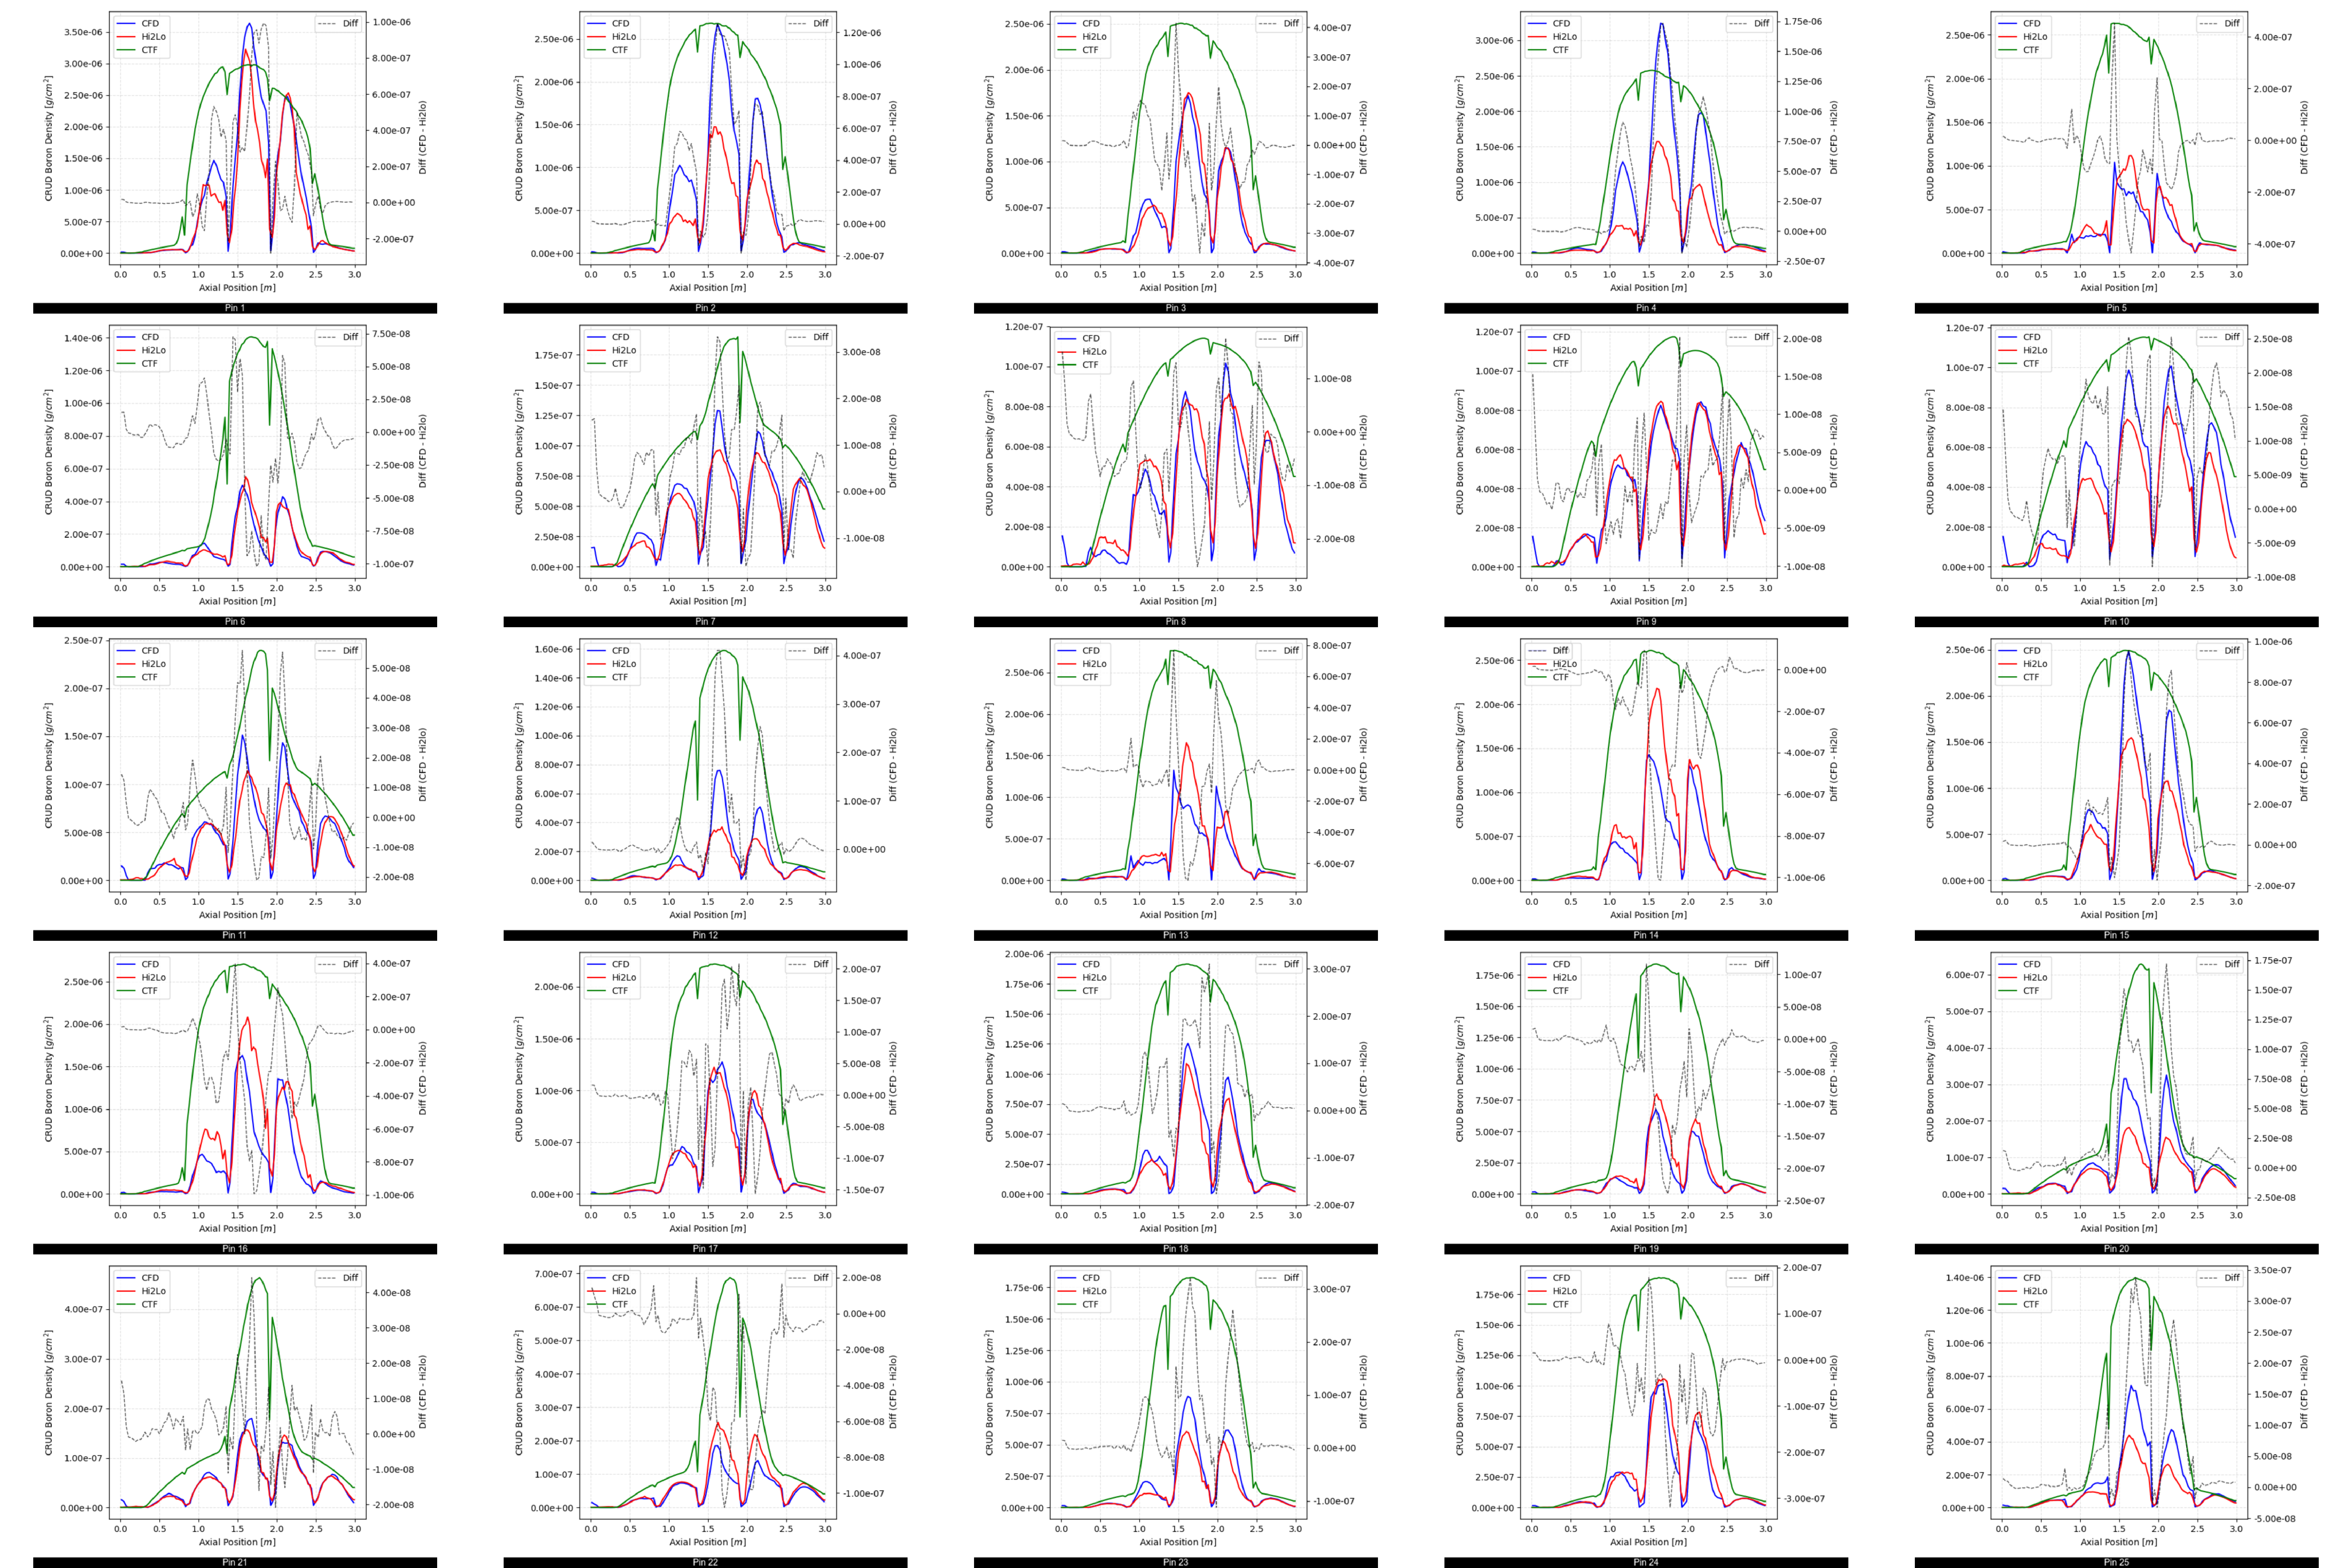
\includegraphics[width=.9\linewidth]{figs/5x5/imp/montage_axial_bmass_sm}
    \caption{5x5 axial crud boron mass results at 300 days.}
    \label{fig:montageaxialbmasssm}
\end{figure}
\begin{figure}[H]
    \centering
    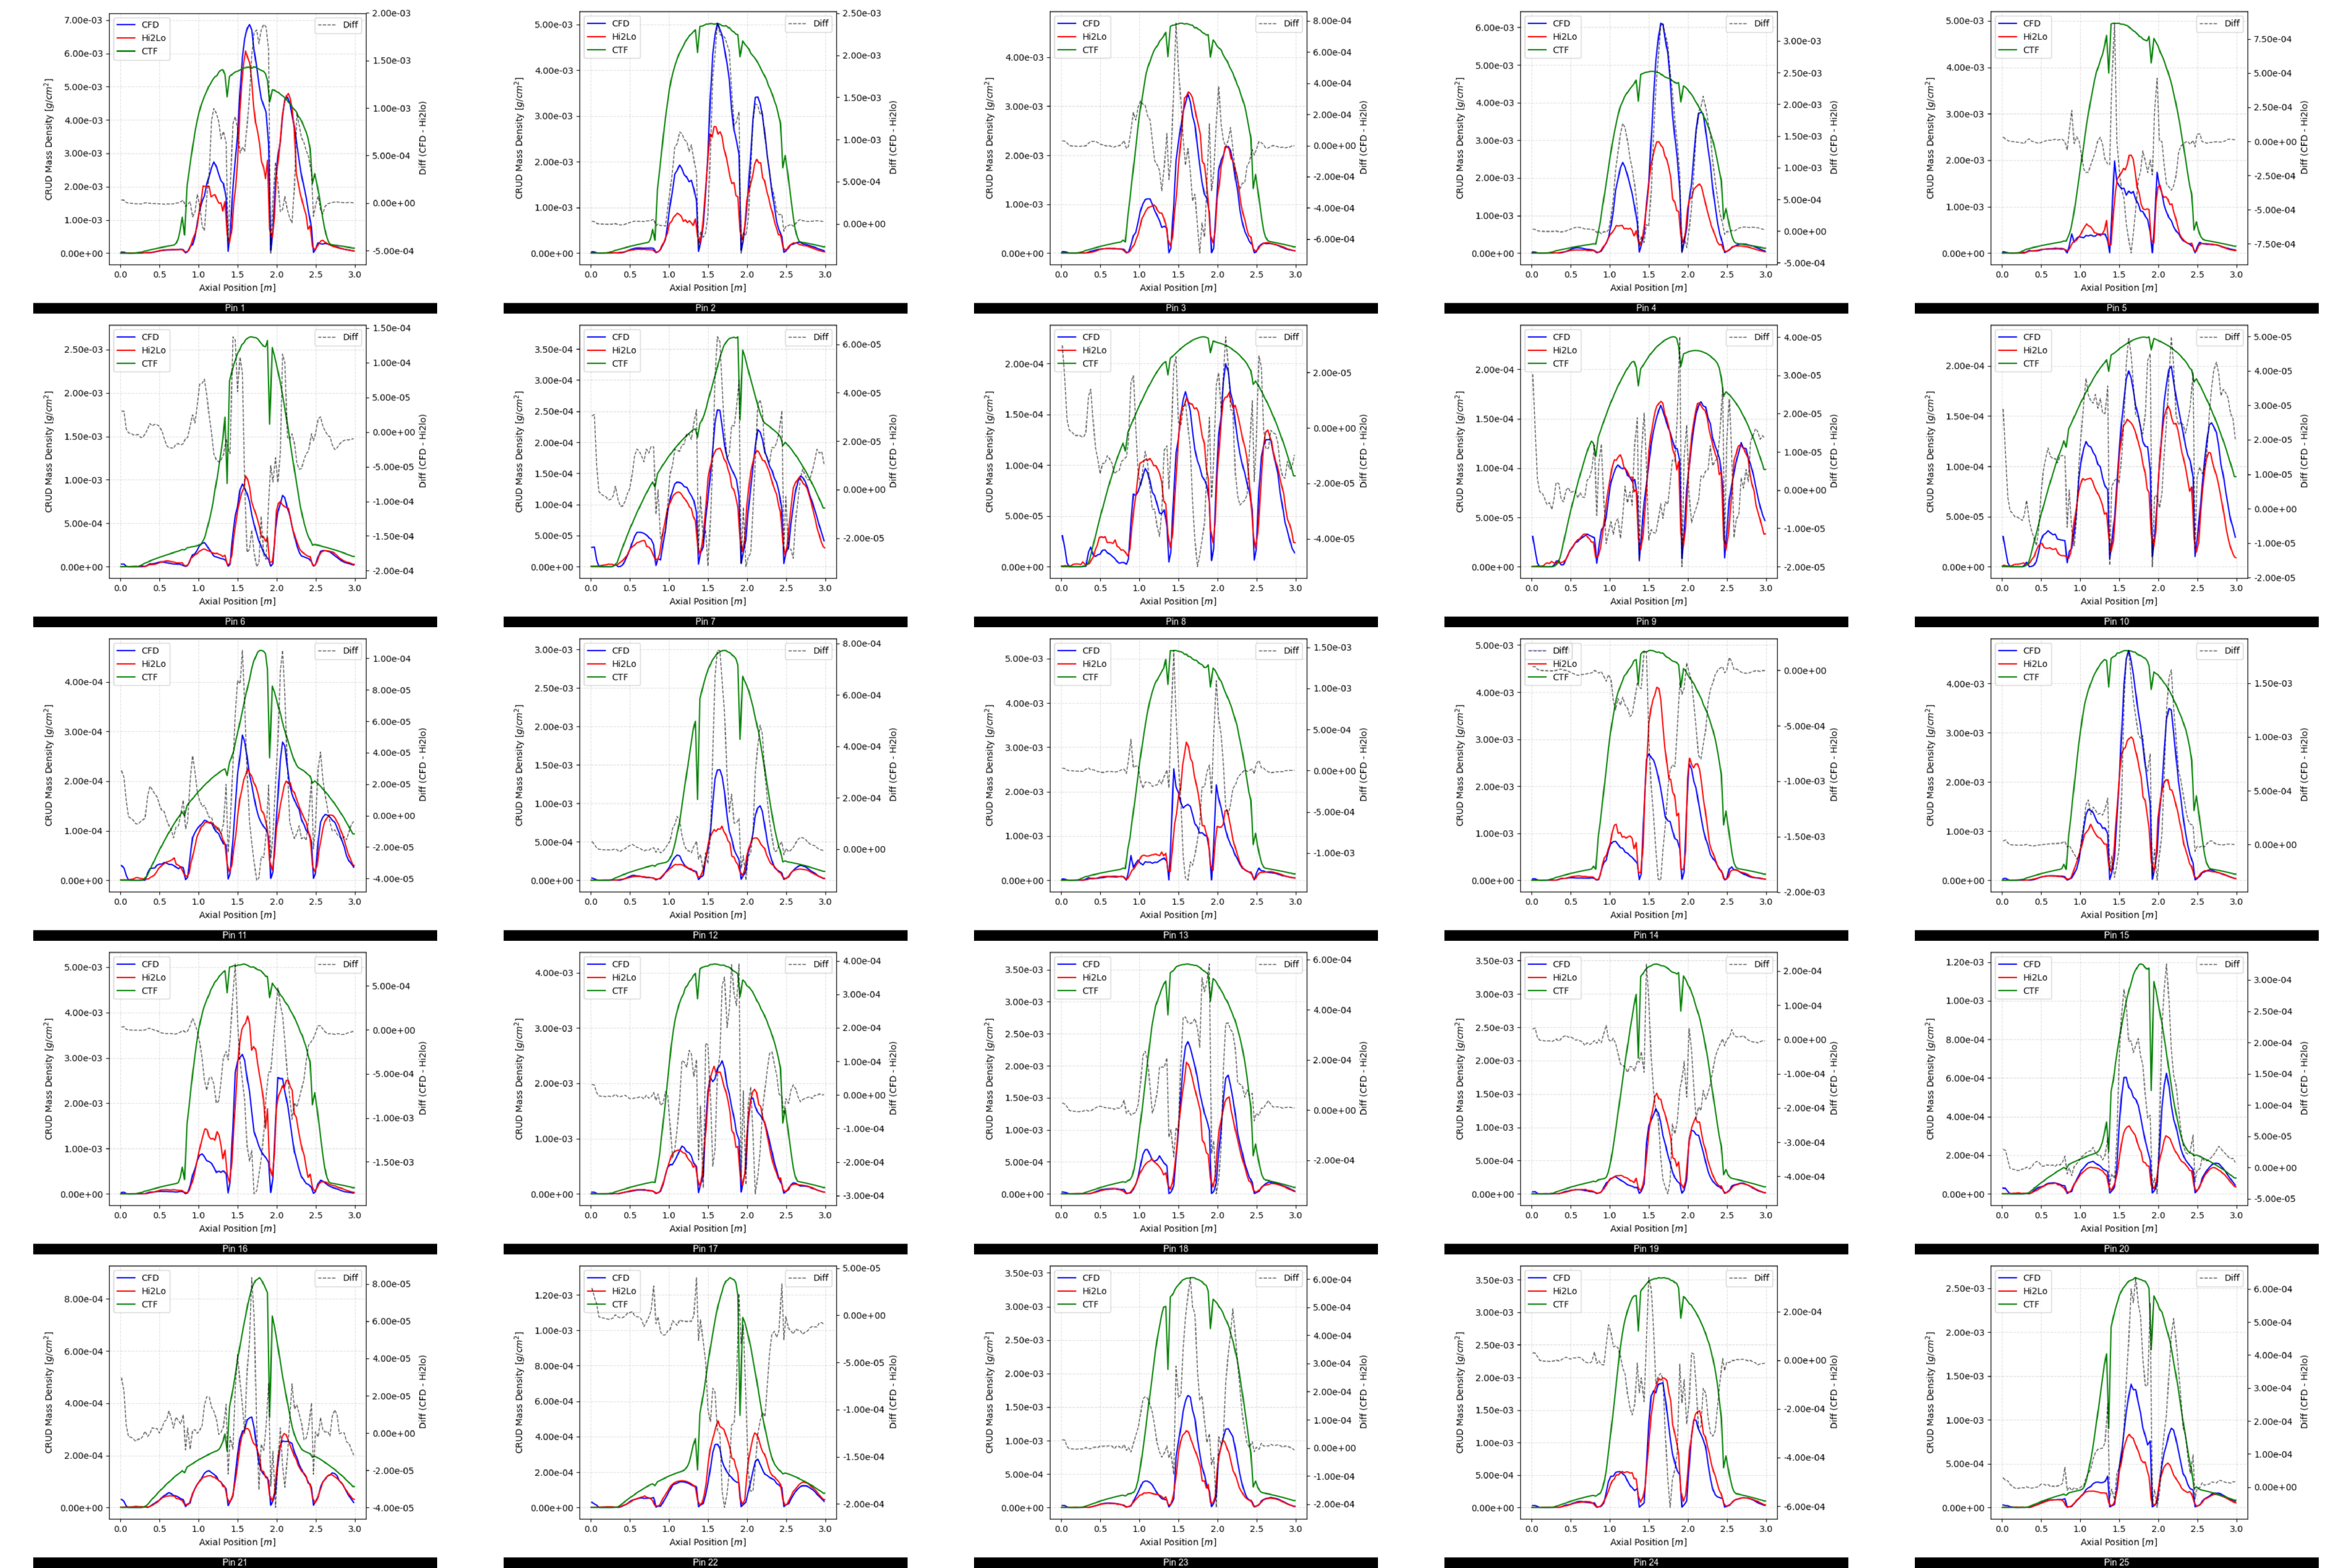
\includegraphics[width=.9\linewidth]{figs/5x5/imp/montage_axial_cmass_sm}
    \caption{5x5 axial crud mass results at 300 days.}
    \label{fig:montageaxialcmasssm}
\end{figure}

\begin{figure}[H]
    \centering
    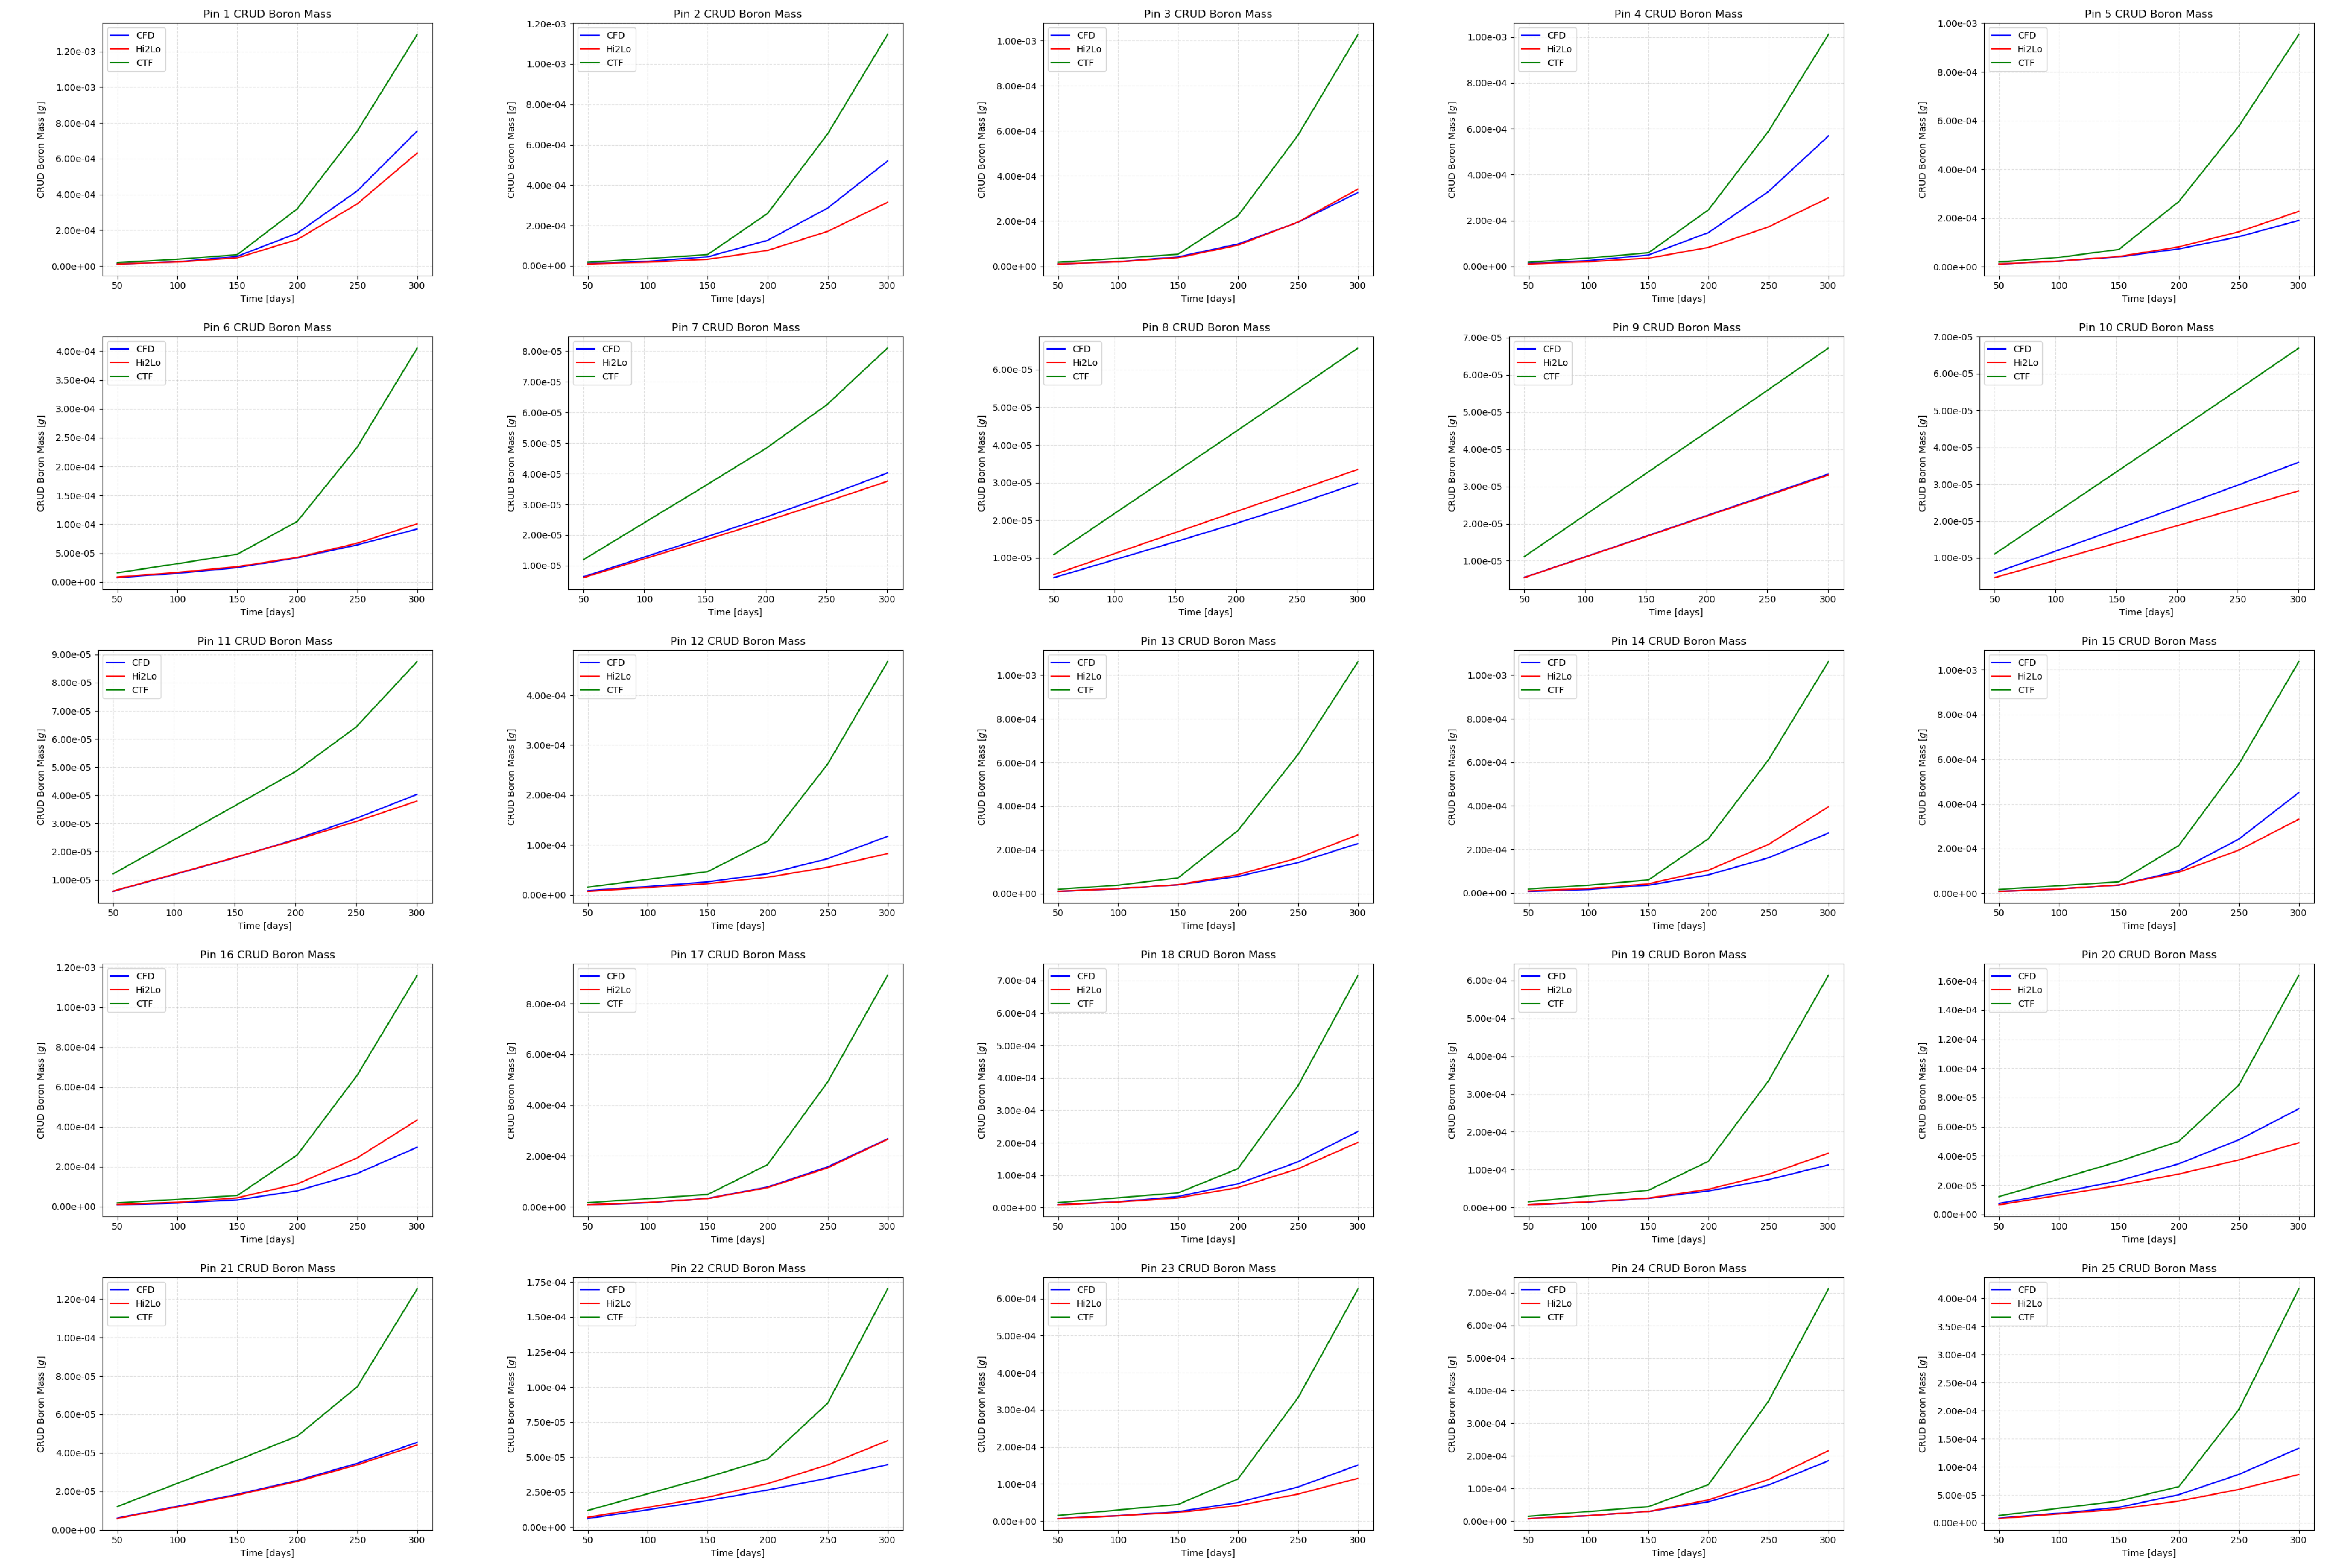
\includegraphics[width=0.9\linewidth]{figs/5x5/imp/montage_time_bmass_sm}
    \caption{5x5 rod integrated crud boron mass vs time.}
    \label{fig:montagetimebmasssm}
\end{figure}


\begin{figure}[H]
    \centering
    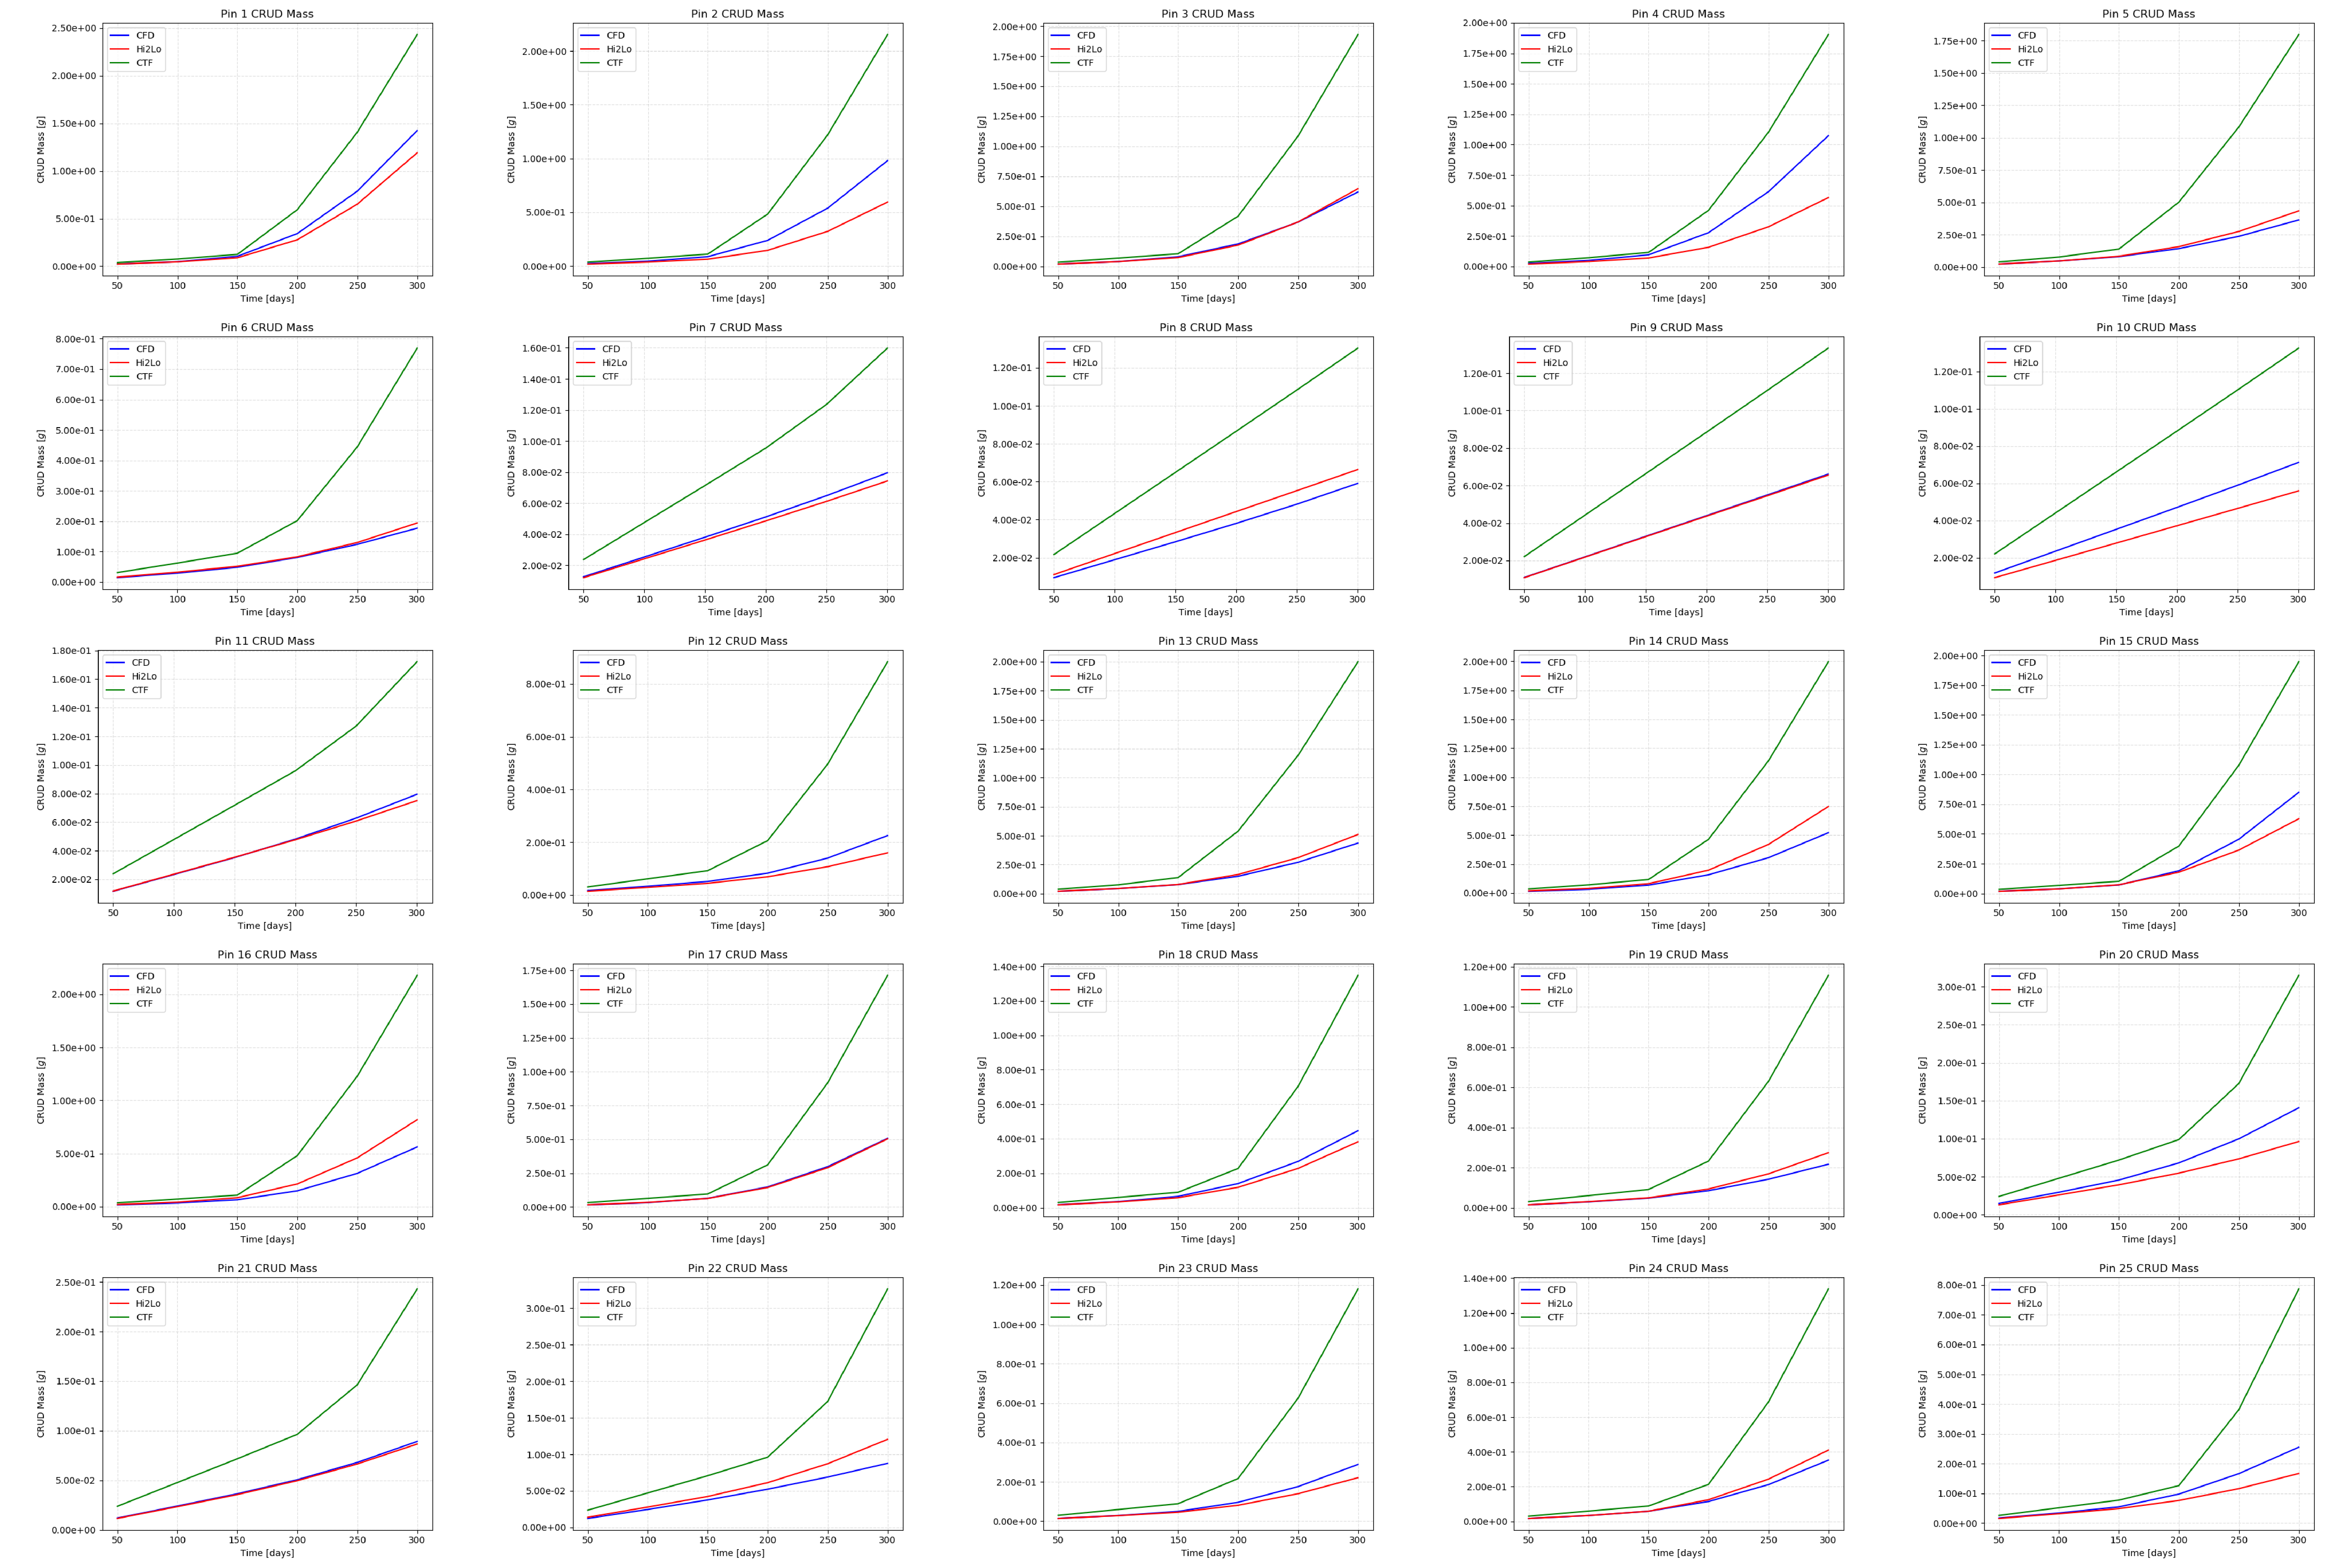
\includegraphics[width=0.9\linewidth]{figs/5x5/imp/montage_time_cmass_sm}
    \caption{5x5 rod integrated crud mass vs time.}
    \label{fig:montagetimecmasssm}
\end{figure}

\end{landscape}



\end{document}
